\documentclass[letterpaper, 11pt]{article}
\usepackage{comment} % enables the use of multi-line comments (\ifx \fi) 
\usepackage{fullpage} % changes the margin
\usepackage{fancyhdr} % for footerhttps://www.overleaf.com/3039851kkndbp#
\usepackage[UKenglish]{isodate}% http://ctan.org/pkg/isodate for date format
\usepackage{float}%force tables/figs into certain placement
\usepackage{changepage}%for dichotomous key
\usepackage{graphicx}%for figures
\usepackage{subcaption}%for figures
\usepackage{hyperref}%for links
\usepackage[font=small,labelfont=bf]{caption}%for captions
\usepackage[letterpaper,margin=1in]{geometry}
\usepackage{natbib}	%for bibliography
\usepackage{placeins}%prevent images from floating into inappropriate sections

\def\labelitemi{--}

\pagestyle{fancy}
\renewcommand{\headrulewidth}{0pt}

\lhead{}
\chead{}
\rhead{}
\lfoot{ENT 432 (Fall 2016) - Penn State}
\cfoot{}
\rfoot{\thepage}
\renewcommand{\footrulewidth}{0.4pt}
\title{Unit 11 - Hymenoptera}
\author{Andrew R. Deans and Istv\'an Mik\'o}

\begin{document}
\cleanlookdateon %removed ordinal date
\maketitle
\thispagestyle{fancy}
\section*{Introduction}
Today we begin looking at a taxon named \textbf{Holometabola}, which all exhibit a form of development called \textbf{holometaboly}. The immature stage (\textbf{larva}) is quite different, usually, from the imago, and the transition to adulthood takes place in a stage we refer to as the \textbf{pupa}. We'll discuss this life cycle in more detail in a later lecture. This lecture focuses on \textbf{Hymenoptera}, a lineage of almost indescribable diversity (155,000 known species and probably at least a million that need names). Is this the largest order? Possibly. These species, commonly known as sawflies, wasps, bees, and ants, exhibit a broad array of morphologies and life histories. Their ecological and economic importance, as predators (\textit{e.g.}, ants), pollinators (bees), pests (\textit{e.g.}, some herbivorous sawflies), and bio-control agents (numerous parasitic wasps) is enormous. 

The predominant parasitoid/predatory lifestyle amongst the derived lineage, Apocrita, is arguably impacted by the appearance of an evolutionary novelty, the wasp waist. The wasp waist separates the locomotory tagma, the mesosoma, from the tagma of reproduction and digestion, the metasoma; it allows for an exceptionally flexible mechanism to maneuver the sting or egg-laying device (ovipositor). Members of this order can be readily separated from other insects based on the following characteristics:

\begin{itemize}
\item haplodiploidy (males are haploid)
\item smaller hind wings connected to larger fore wings by hook-like spurs (hamuli) (Figure \ref{fig:hamuli})
\item transverse and longitudinal veins cannot be differentiated (compare with Odonata and Plecoptera, \textit{e.g.}, where transverse veins are usually less sclerotized and more flexible than longitudinal veins)
\item protibial apical spur and the first basitarsus is modified into an antenna cleaning device
\item abdominal tergite I at least partly fused with metanotum
\end{itemize}

\subsection*{Big picture questions}
Given what you read and discussed in lecture, what adaptations contributed to such a large radiation? How does this diversity look phylogenetically?\\

\noindent{}How do \textbf{idiobiont} parasitoids differ from \textbf{koinobiont}s?\\

\noindent{}Familiarize yourself with the following taxon names, which refer to organisms you are likely to encounter in the northeastern USA and/or which are phylogenetically relevant. Can you describe how these arthropods live (natural history) and roughly how diverse they are? Do you know how they're related to one another? If you had to choose a family to study from the taxa below which one would it be and why?

\begin{enumerate} 
\item Apocrita
\item Aculeata
\end{enumerate}

\begin{figure}[ht!]
  \centering
    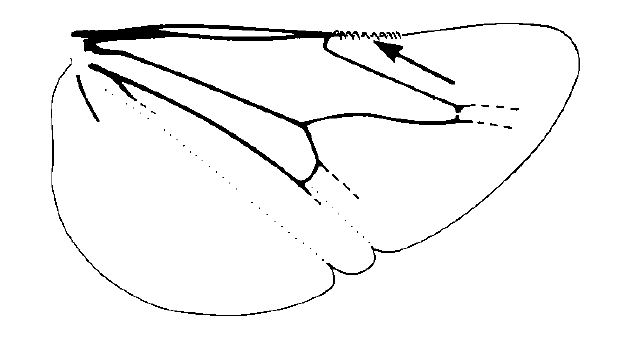
\includegraphics[width=0.35\textwidth]{Hamuli}
  \caption{Hind wing with hamuli (arrow) \citep[][pg. 42]{goulet1993hymenoptera}}
  \label{fig:hamuli}
\end{figure}

\section*{Materials}
\begin{itemize}
\item specimens (provided)
\item fine forceps, probes (provided)
\item sorting tray, watch glasses, gloves, safety glasses, glycerine, ethanol (provided)
\item pencil/paper for sketches
\end{itemize}

\section*{Safety}
We will be working with sharp tools and insects on pins. Wear your personal protective gear at all times. Specimens are to be returned to their vials after lab, and glycerine and ethanol will be collected for proper disposal or reuse.

\section*{Methods}
Working with a partner, organize your space, specimens, tools, and microscope. Use your probe and forceps to manipulate the specimen. In this lab, however, we will not be dissecting specimens (unless otherwise noted). You can start anywhere in the handout.

\section{Hymenoptera}
\subsection{Non-apocritan Hymenoptera (``Symphyta'')}
\begin{itemize}
\item Body in dorsal view with very little or no constriction near its middle between abdominal segments 1 and 2 (“wasp waist” absent)
\item cenchrus usually present (arrows in Figure \ref{fig:symphyt1})
\item fore tibia with two apical spurs
\item never less than 3 mm in length
\item first abdominal tergite usually divided medially
\end{itemize}

\begin{figure}[ht!]
  \centering
    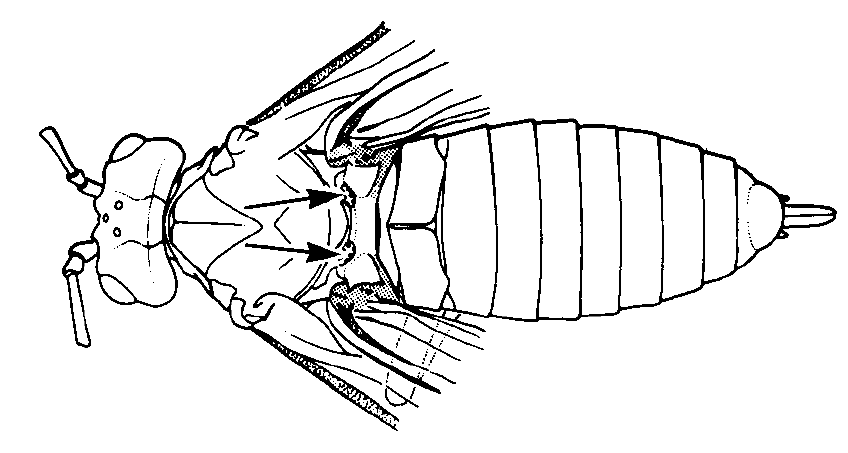
\includegraphics[width=0.5\textwidth]{SymphytaHabitus}
  \caption{Symphytan dorsal habitus \citep[][pg. 42]{goulet1993hymenoptera}}
  \label{fig:symphyt1}
\end{figure}

\subsubsection{Xyelidae}
\begin{itemize}
\item antennae with less than 10 flagellomeres
\item first flagellum much longer than following flagellomeres  
\item maxillary palp leg-like
\item fore wing with 3 marginal cells (MC) and distinct subcostal vein (Sc) (Figure \ref{fig:xyelidwings})
\item three veins along the anteroproximal margin of fore wing connecting pterostigma with wing base
\end{itemize}

\begin{figure}[ht!]
    \centering
    \begin{subfigure}[ht!]{0.4\textwidth}
        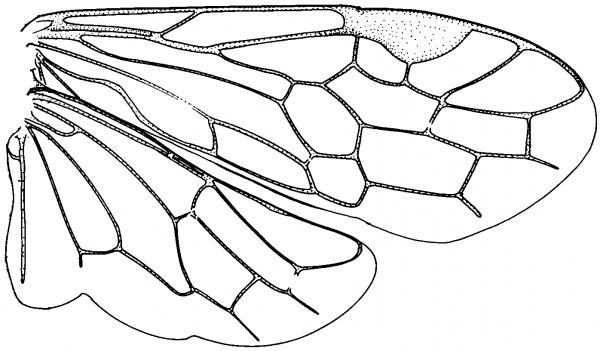
\includegraphics[width=\textwidth]{XyelidWings}
        \caption{Wings \citep[][modified from Fig. 32]{goulet1993hymenoptera}}
        \label{fig:xyelidwings}
    \end{subfigure}
    \hfill 
    \begin{subfigure}[ht!]{0.42\textwidth}
        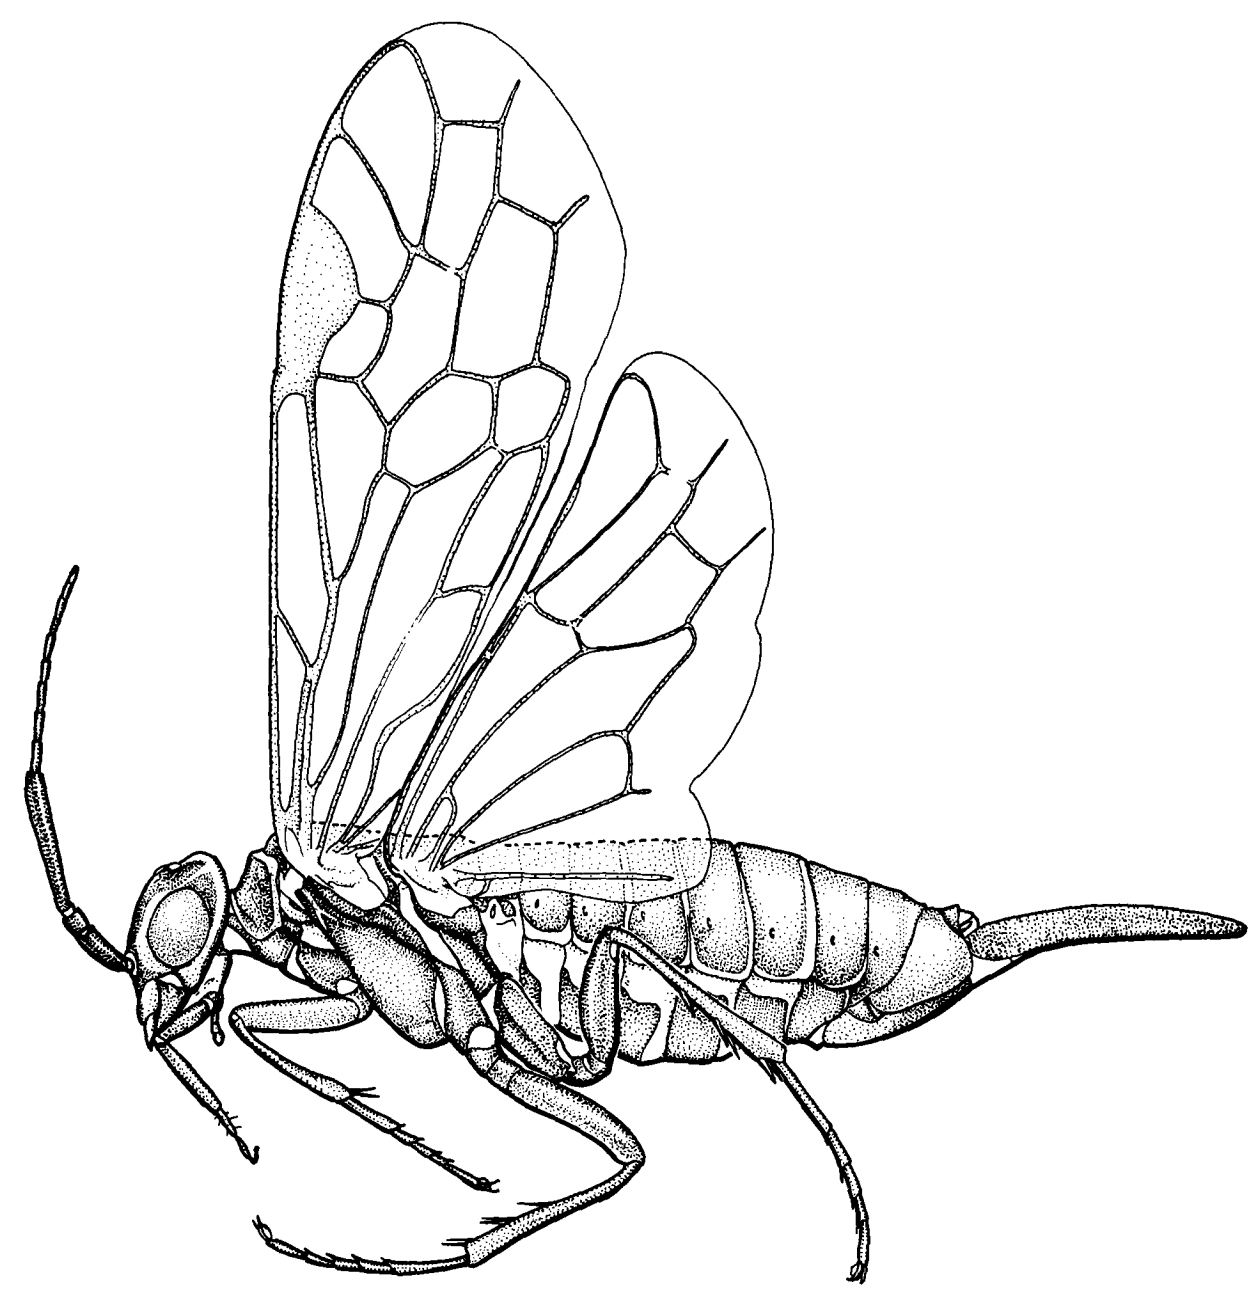
\includegraphics[width=\textwidth]{XyelidHabitus}
        \caption{Habitus \citep[][Fig. 32]{goulet1993hymenoptera}}
        \label{fig:xyelidhead}
    \end{subfigure}
    \caption{Xyelidae}\label{fig:xyelid1}
\end{figure}

\subsubsection{Argidae (argid sawflies)}
\begin{itemize}
\item antenna with 1 flagellomere (Figure \ref{fig:argid1})
\item mesonotum is not divided by a straight transverse groove
\item fore wing with less than 2 marginal cells
\item two veins along the anteroproximal margin of fore wing connecting pterostigma with wing base
\end{itemize}

\begin{figure}[ht!]
    \centering
    \begin{subfigure}[ht!]{0.11\textwidth}
        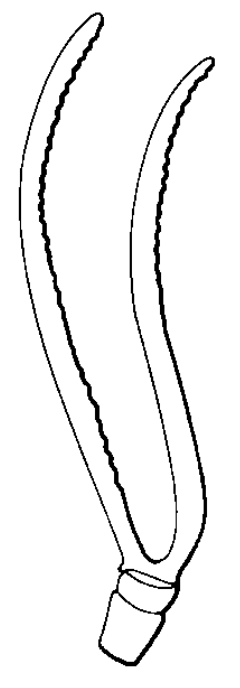
\includegraphics[width=\textwidth]{ArgidAntenna}
        \caption{Antenna}
        \label{fig:argid1}
    \end{subfigure}
    \qquad
    \begin{subfigure}[ht!]{0.45\textwidth}
        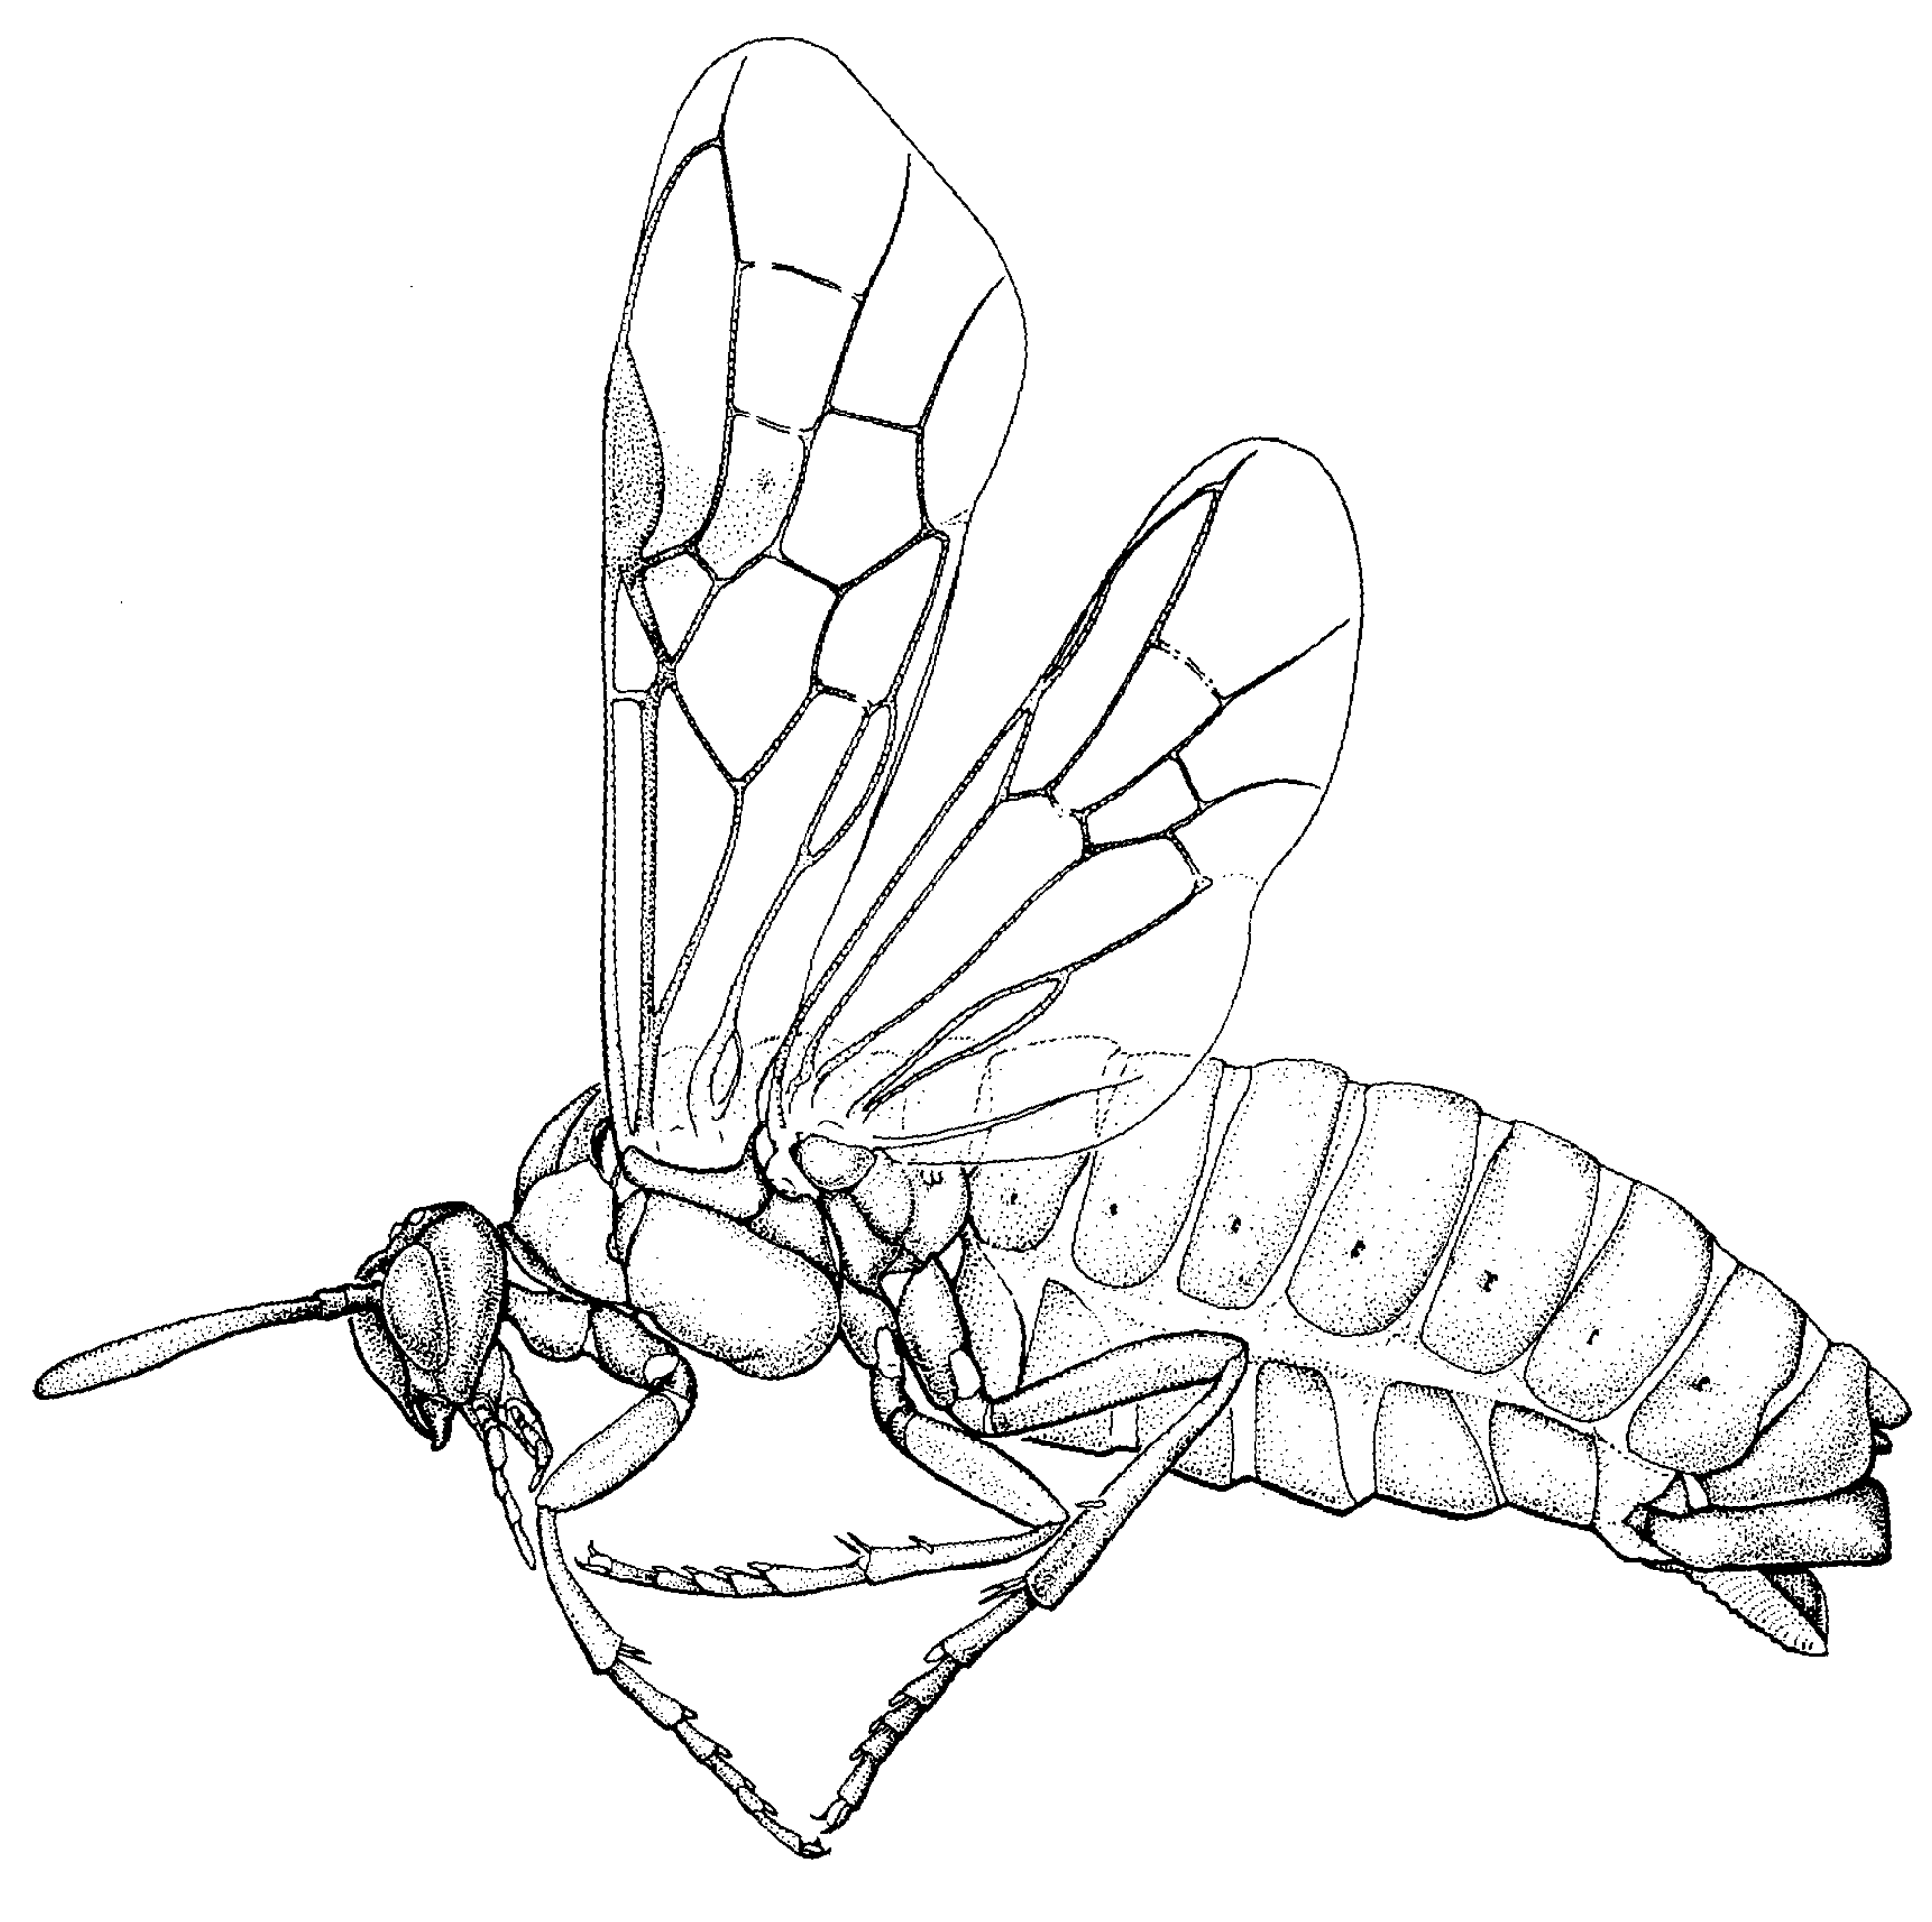
\includegraphics[width=\textwidth]{ArgidHabitus}
        \caption{Habitus}
        \label{fig:argid2}
    \end{subfigure}
    \caption{Argidae \citep[][pg. 106 (a) and Fig. 26 (b)]{goulet1993hymenoptera}}\label{fig:argid}
\end{figure}

\subsubsection{Diprionidae (conifer sawflies)}
\begin{itemize}
\item antennae with approximately 20 flagellomeres, comb-like in males and saw-like in females
% * <carolyntrietsch@gmail.com> 2015-10-05T19:18:35.756Z:
%
%  write that one imag is a female, one is male, and ask why there are enlarged surfaces on the antennae?
%
\item fore wing with less than 2 marginal cells
\item two veins along the anteroproximal margin of fore wing connecting pterostigma with wing base
\end{itemize}
\noindent{}Why do you think males have pectinate antennae?

\begin{figure}[ht!]
    \centering
    \begin{subfigure}[ht!]{0.14\textwidth}
        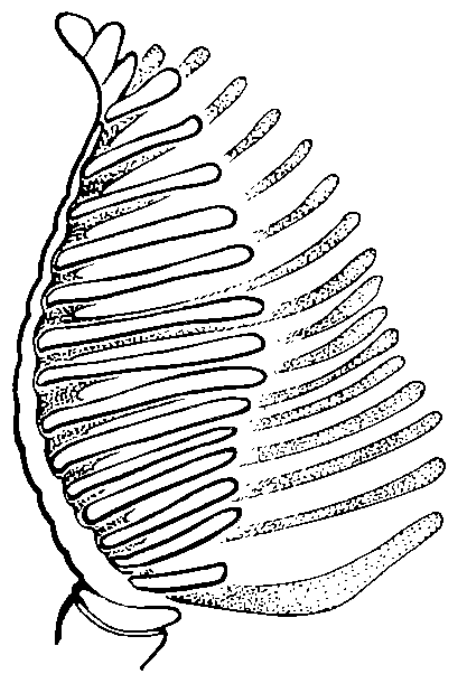
\includegraphics[width=\textwidth]{DiprionidAntenna}
        \caption{Male antenna}
        \label{fig:diprionid1}
    \end{subfigure}
    \qquad
    \begin{subfigure}[ht!]{0.45\textwidth}
        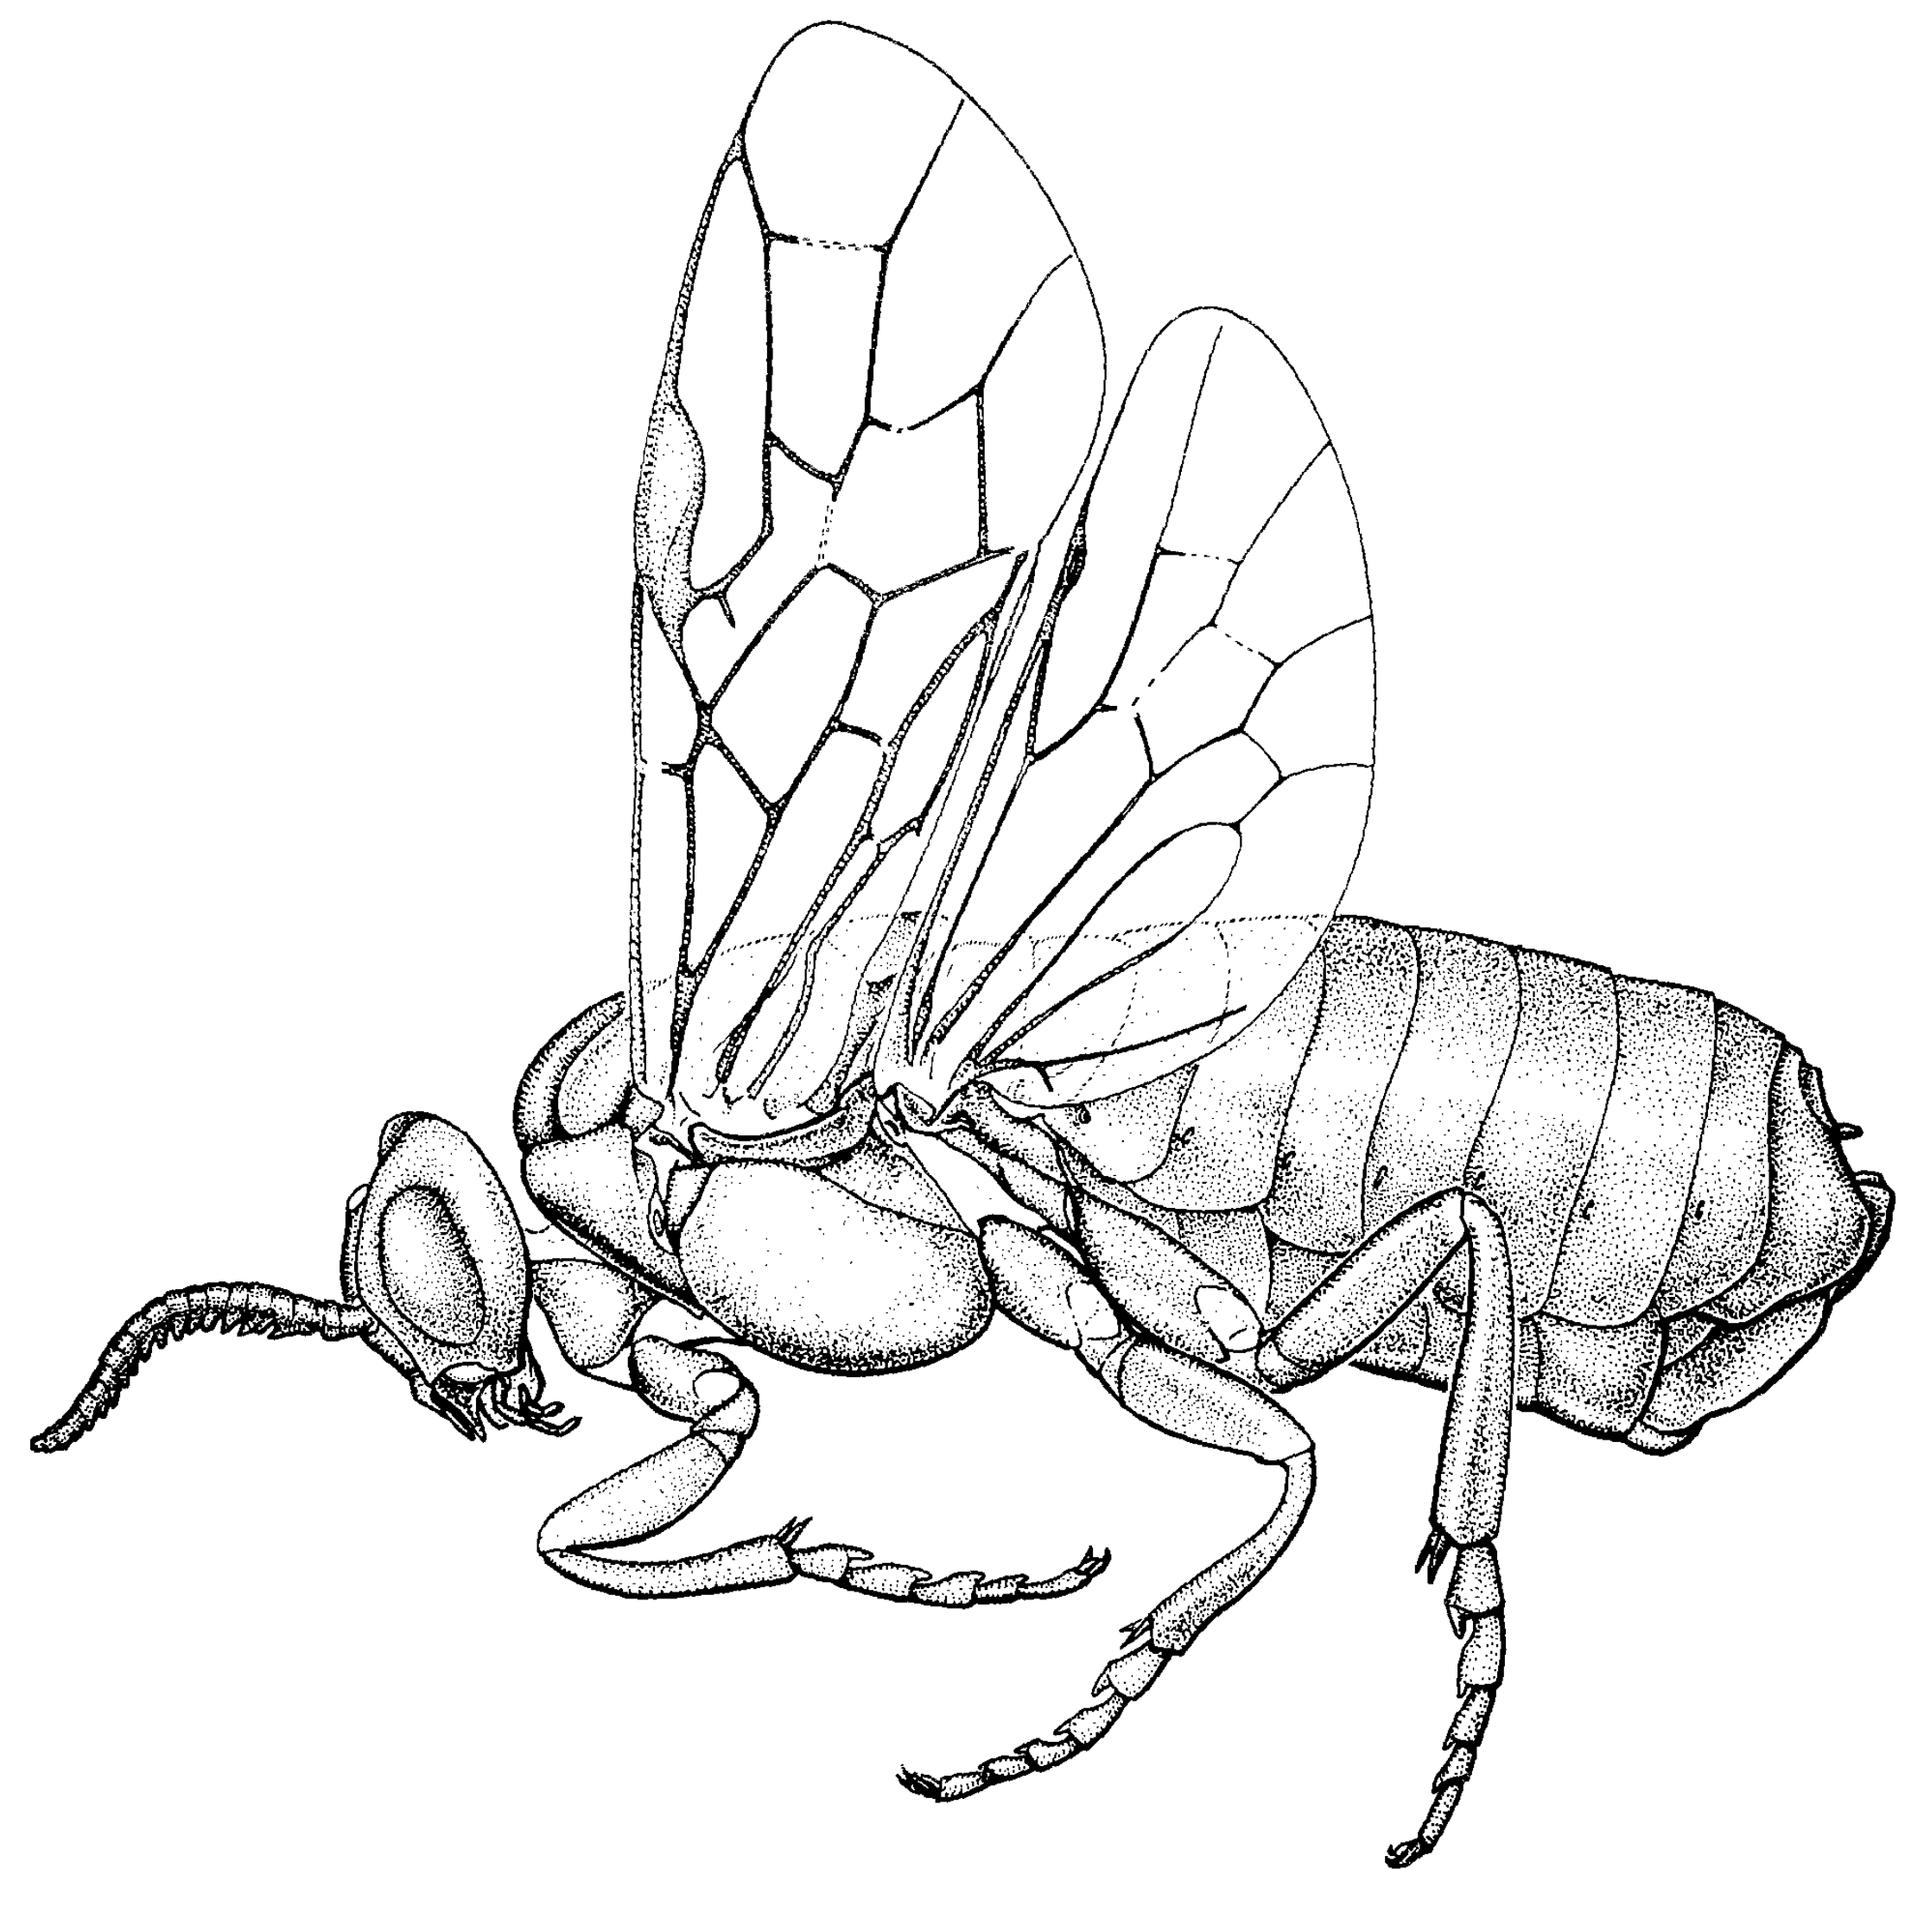
\includegraphics[width=\textwidth]{DiprionidHabitus}
        \caption{Habitus, male (left) and female (right)}
        \label{fig:diprionid2}
    \end{subfigure}
    \caption{Diprionidae \citep[][pg. 108 (a) and Fig. 29 (b)]{goulet1993hymenoptera}}\label{fig:diprion}
\end{figure}

\subsubsection{Tenthredinidae (common sawflies)}
\begin{itemize}
\item antennae with 3--7 flagellomeres (Figure \ref{fig:tenthred1})
\item first abdominal tergum clearly separated from metapleuron
\end{itemize}

\begin{figure}[ht!]
  \centering
    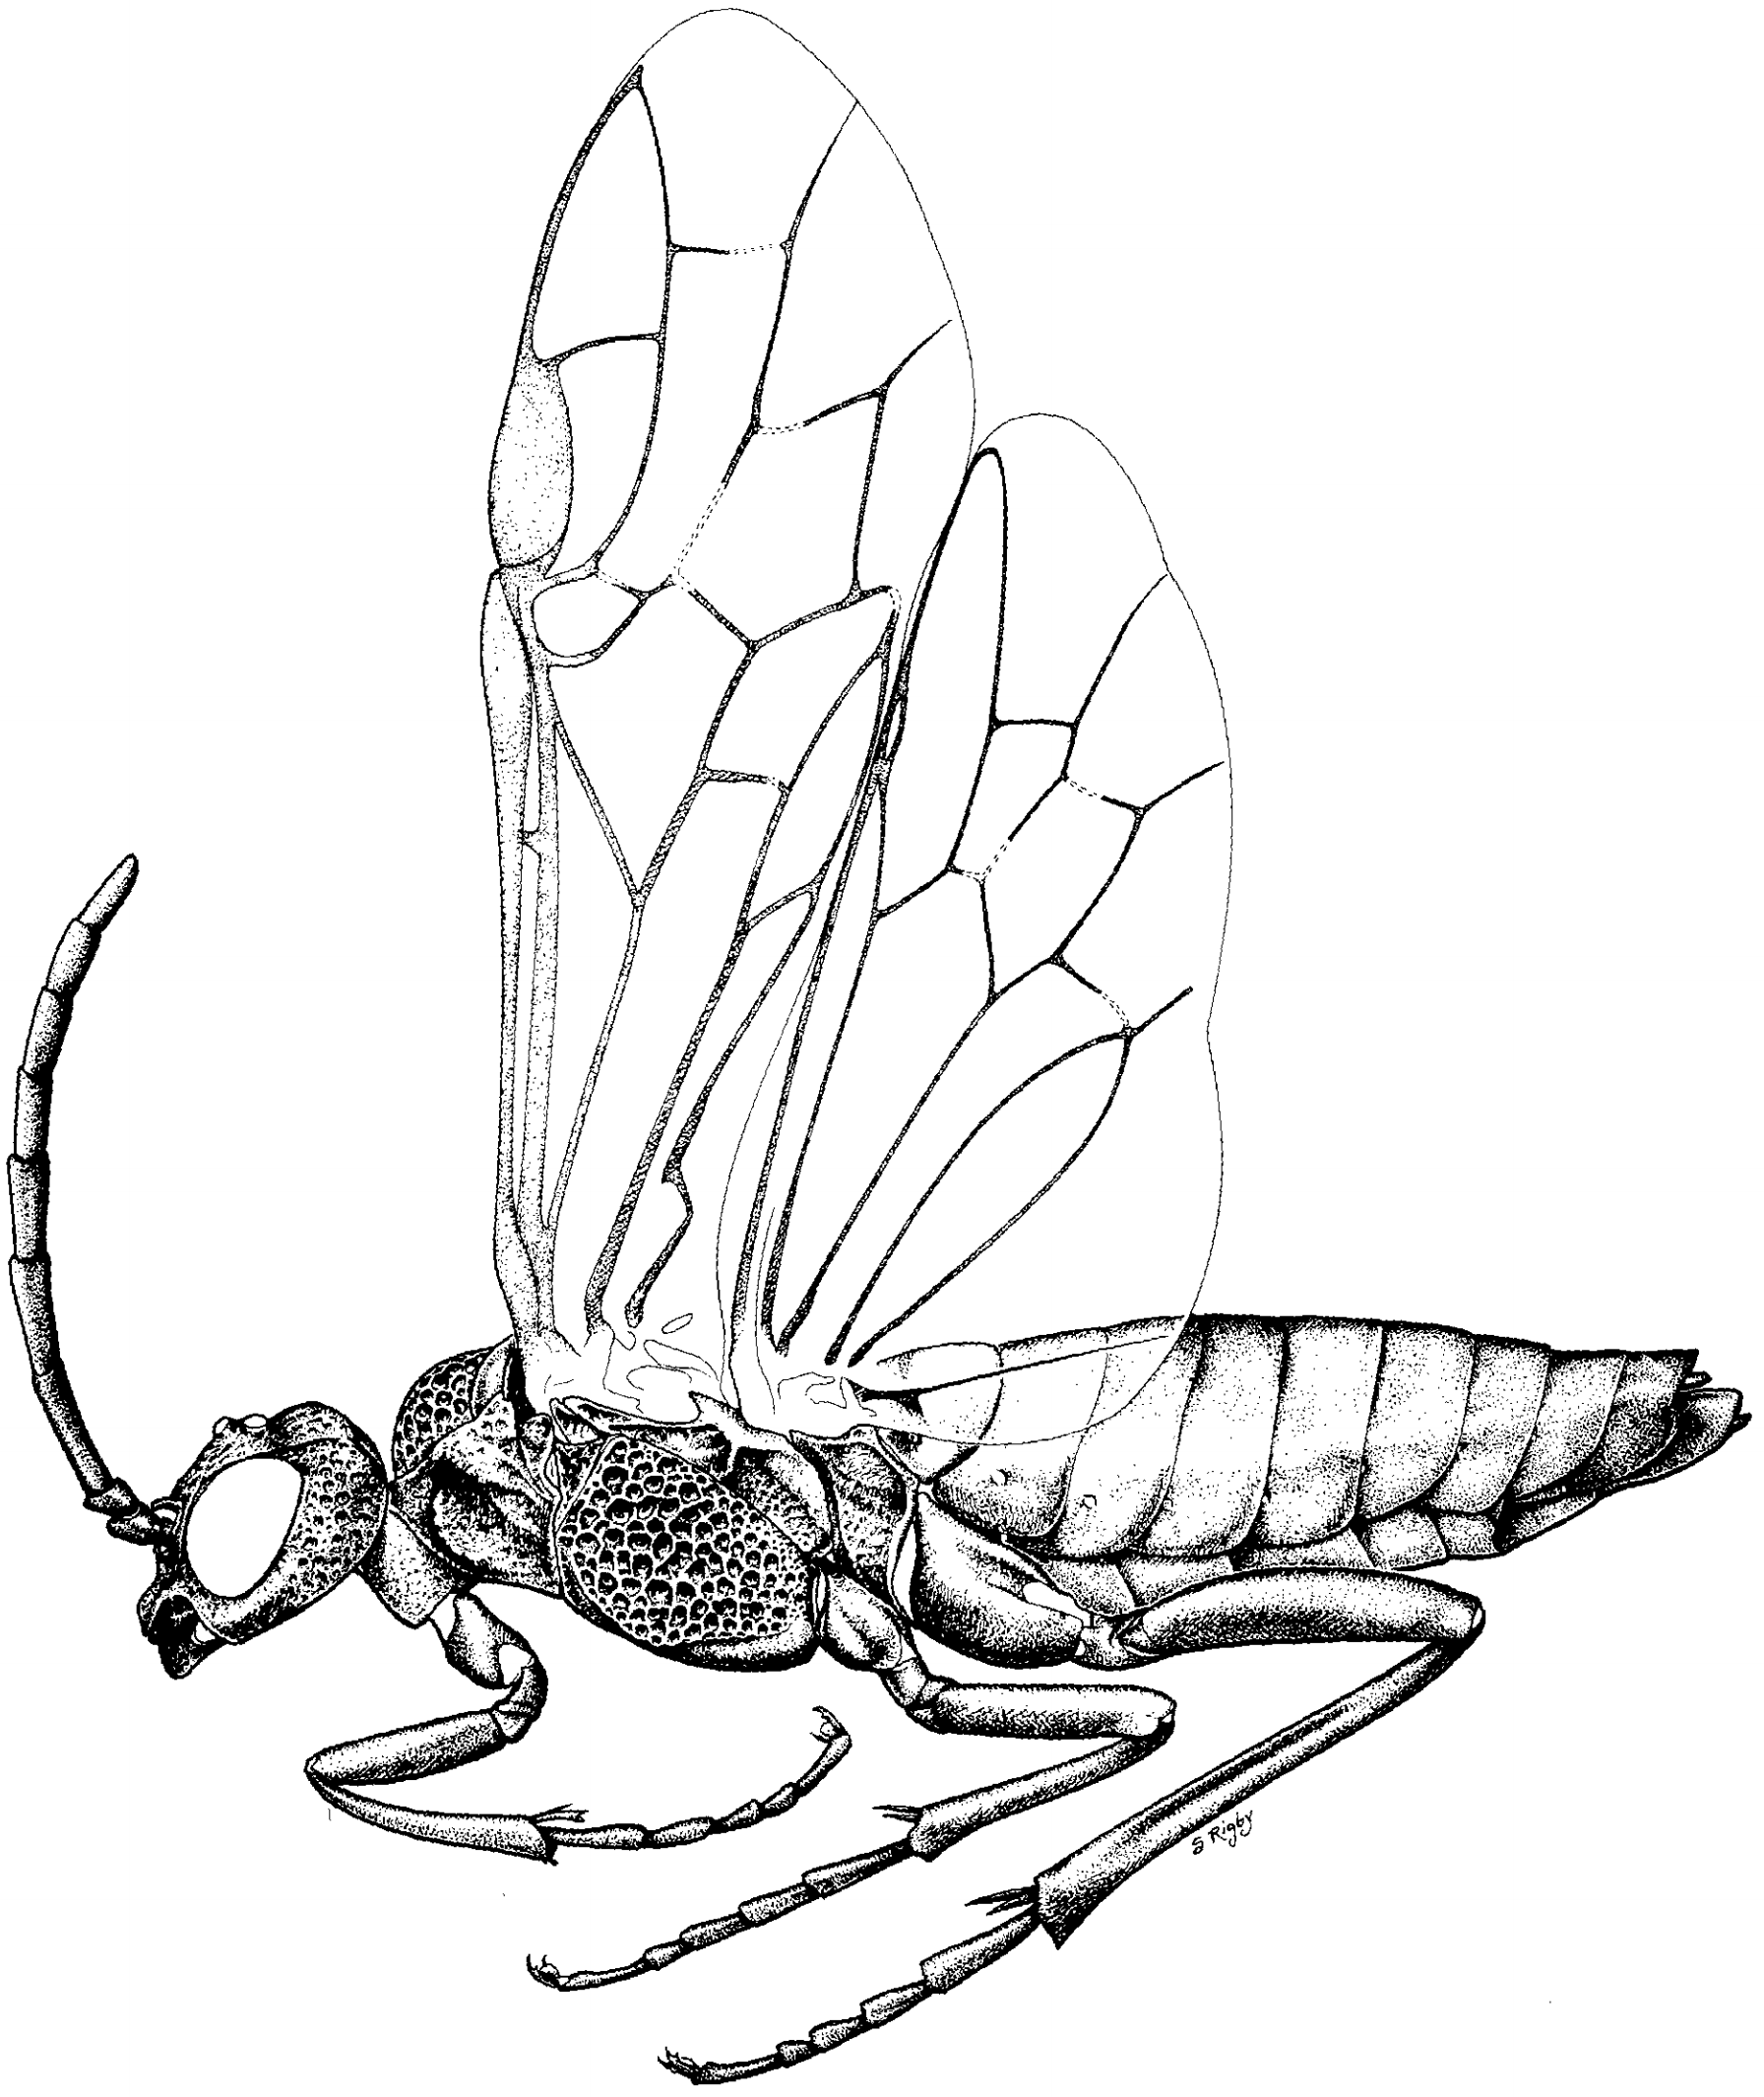
\includegraphics[width=0.4\textwidth]{TenthredinidHabitus}
  \caption{Tenthredinidae, lateral habitus \citep[][Fig. 31]{goulet1993hymenoptera}}
  \label{fig:tenthred1}
\end{figure}

\noindent{}The next two families represent a transition in life history, from larvae feeding on leaves to larvae feeding inside wood (\textit{i.e.}, they are wood-boring insects). Can you see evidence of this transition in the external morphology of these hymenopterans? Compare these next two taxa to Tenthredinidae or Argidae, for example, and describe or illustrate a few differences. What is the function of the transcutal articulation?

\subsubsection{Siricidae (horntails)}
\begin{itemize}
\item antennae with \textgreater{}20 flagellomeres
\item pronotum with a large dorsal (horizontal) surface (Figure \ref{fig:siricid1})
\item fore tibia with one apical spur
\item last tergum in females and last sternum in males with apical cylindrical projection (Figure \ref{fig:siricid2})
\end{itemize}
\noindent{}Female siricids have pockets (``mycangia''; we'll see this word again when we cover Coleoptera) at the base of their ovipositors that contain fungi. What do you think is the role of these fungi?

\begin{figure}[ht!]
    \centering
    \begin{subfigure}[ht!]{0.4\textwidth}
        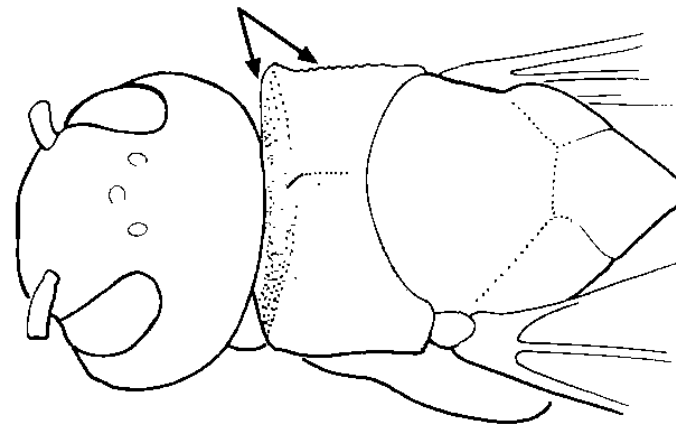
\includegraphics[width=\textwidth]{SiricidPronotum}
        \caption{Siricidae, dorsal head and thorax \citep[][pg. 70]{goulet1993hymenoptera}}
        \label{fig:siricid1}
    \end{subfigure}
    \hfill
    \begin{subfigure}[ht!]{0.45\textwidth}
        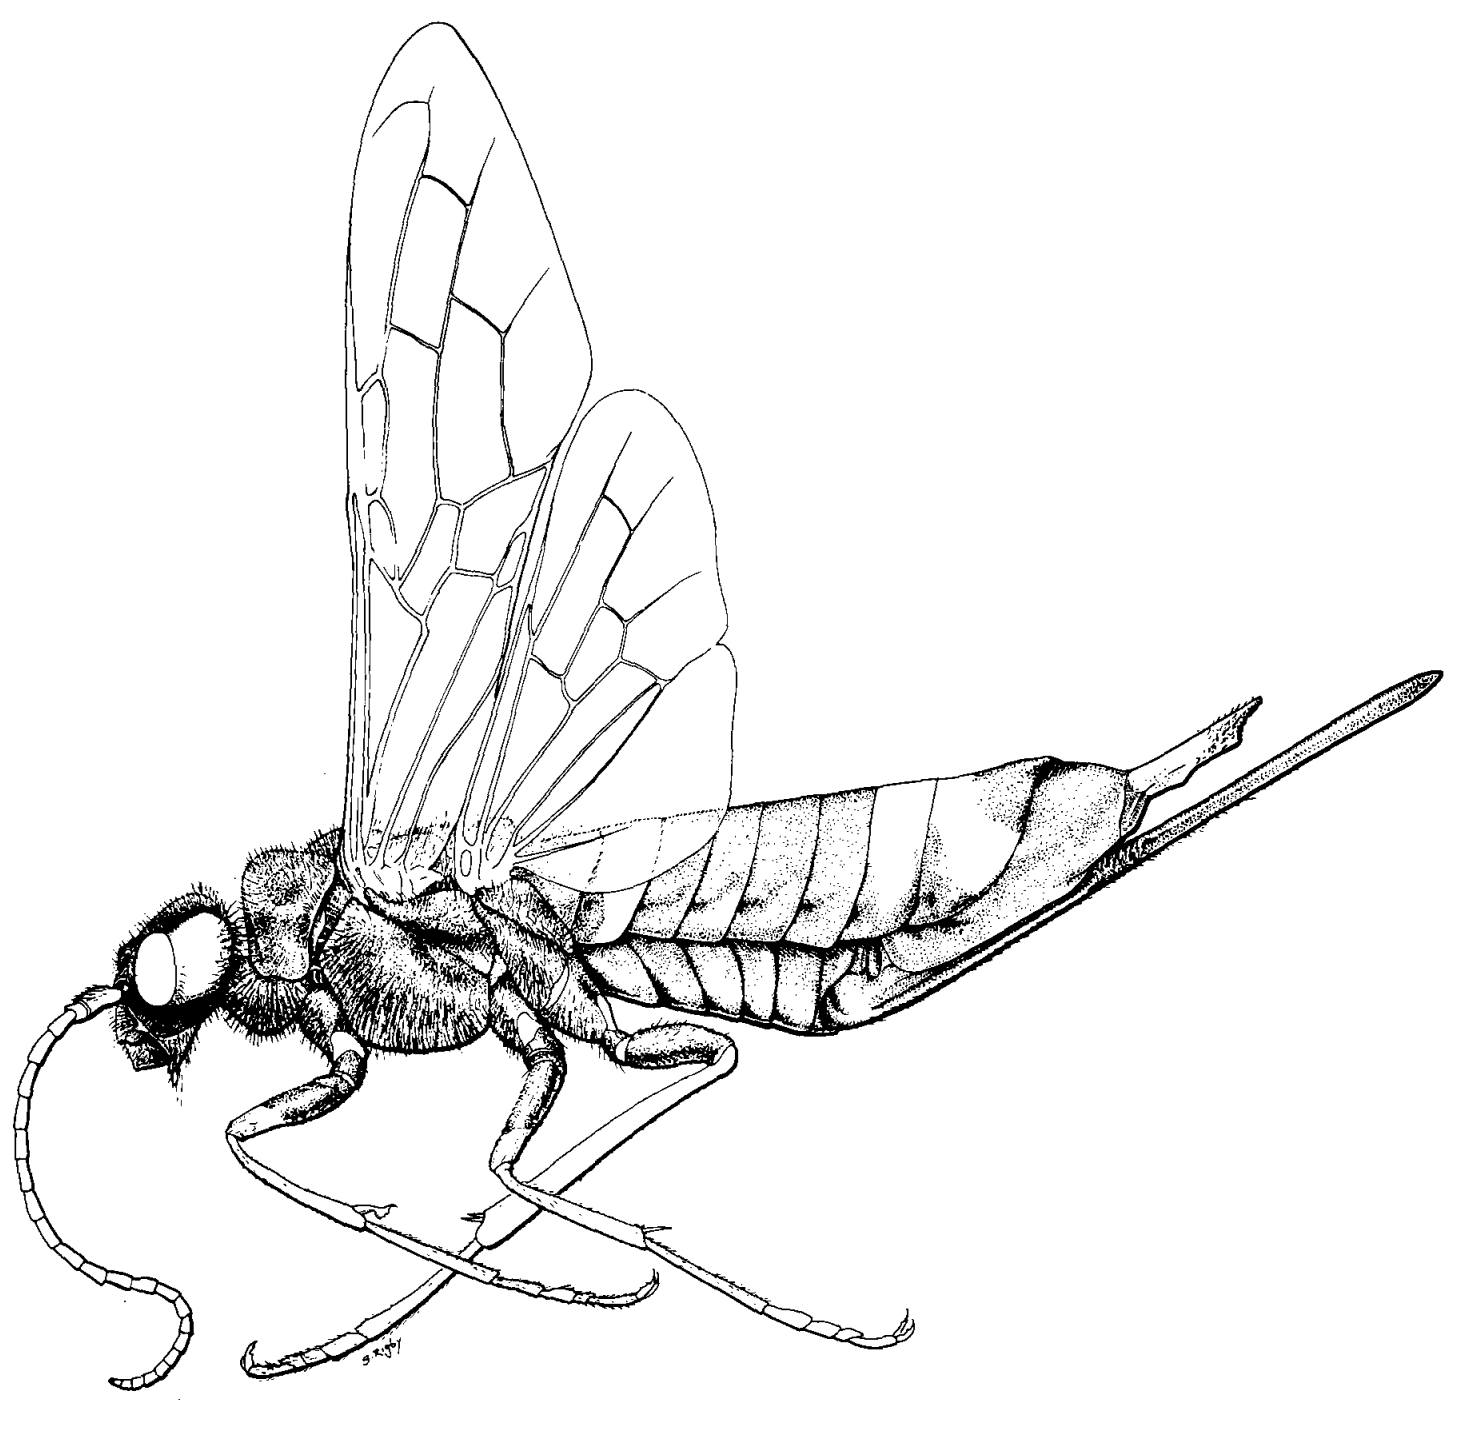
\includegraphics[width=\textwidth]{SiricidHabitus}
        \caption{Habitus \citep[][Fig. 25]{goulet1993hymenoptera}}
        \label{fig:siricid2}
    \end{subfigure}
    \caption{Siricidae}\label{fig:siricids}
\end{figure}

\subsection{Apocrita}
The remaining hymenopterans comprise the megadiverse Apocrita, a lineage characterized in part, at least ancestrally, by developing as parasitoids of other insects. In dorsal view, the body has a distinct constriction near its middle (\textit{i.e.}, ``wasp waist'' present); note that the middle tagma is referred to as the ``mesosoma'' and the posteriormost tagma is the ``metasoma''. 

\subsubsection{Braconidae}
\begin{itemize}
\item antenna usually with 16 or more antennomeres (Figure \ref{fig:braconid1})
\item fore wing C + Sc + R fused (\textit{i.e.}, anterior margin of wing with relatively thick wing vein)
\item pterostigma usually present 
\item one recurrent vein or none (Figure \ref{fig:braconid2} arrow) 
\item no ``horse head'' cell (compare with Ichneumonidae)
\item first and second metasomal segments often fused and immobile dorsally 
\end{itemize}

\begin{figure}[ht!]
    \centering
    \begin{subfigure}[ht!]{0.55\textwidth}
        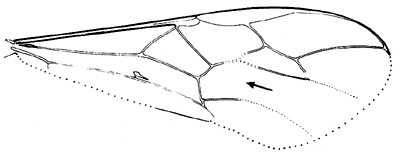
\includegraphics[width=\textwidth]{BraconidWing}
        \caption{Fore wing \citep[][pg. 359]{goulet1993hymenoptera}}
        \label{fig:braconid1}
    \end{subfigure}
    \hfill
    \begin{subfigure}[ht!]{0.38\textwidth}
        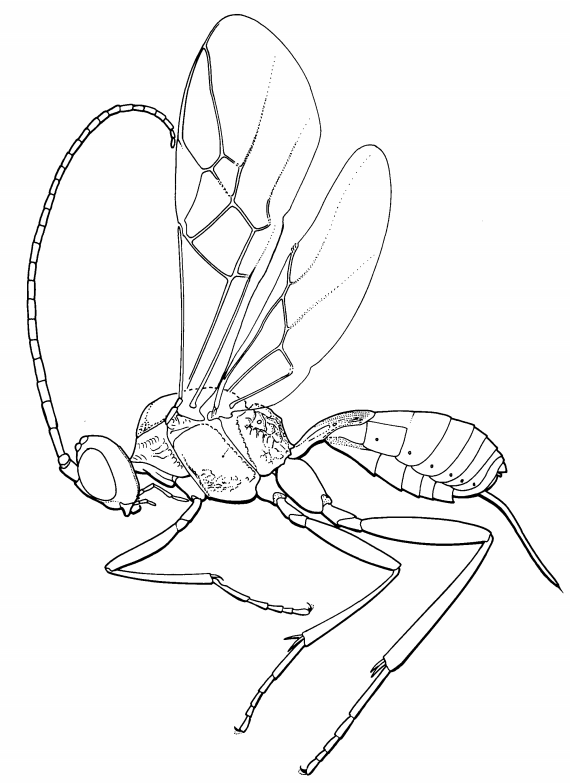
\includegraphics[width=\textwidth]{BraconidHabitus}
        \caption{Lateral habitus \citep[][Fig. 138]{goulet1993hymenoptera}}
        \label{fig:braconid2}
    \end{subfigure}
    \caption{Braconidae}\label{fig:braconids}
\end{figure}

\subsubsection{Ichneumonidae (ichneumon wasps)}
\begin{itemize}
\item antenna usually with 16 or more antennomeres
\item fore wing C + Sc + R fused (\textit{i.e.}, anterior margin of wing with relatively thick wing vein)
\item pterostigma usually present
\item two recurrent veins present (Figure \ref{fig:ichneumonid1} arrow)
\item ``horse head cell'' present (often not quite horse-like)
\item first and second metasomal segments not fused 
\end{itemize}

\begin{figure}[ht!]
    \centering
    \begin{subfigure}[ht!]{0.5\textwidth}
        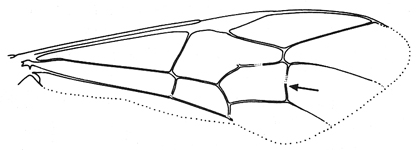
\includegraphics[width=\textwidth]{IchneumonidWing}
        \caption{Fore wing \citep[][pg. 359]{goulet1993hymenoptera}}
        \label{fig:ichneumonid1}
    \end{subfigure}
    \hfill
    \begin{subfigure}[ht!]{0.46\textwidth}
        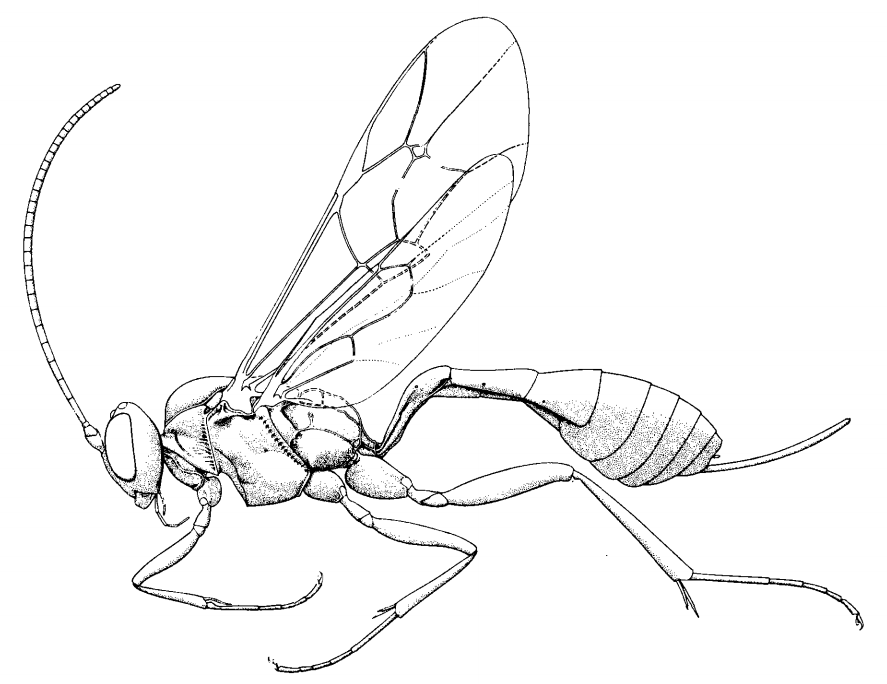
\includegraphics[width=\textwidth]{IchneumonidHabitus}
        \caption{Lateral habitus \citep[][Fig. 159]{goulet1993hymenoptera}}
        \label{fig:ichneumonid2}
    \end{subfigure}
    \caption{Braconidae}\label{fig:ichneumonids}
\end{figure}

\subsubsection{Evaniidae (ensign or hatchet wasps)}
\begin{itemize}
\item antenna with 13 antennomeres (one neotropical genus has 10)
\item pterostigma relatively small
\item metasoma arising dorsally on mesosoma, distance between propodeal foramen and metacoxal cavity much larger than width of either opening
\item metasoma hatchet shaped or flag-shaped
\item first and second metasomal segments often fused and immobile dorsally 
\item petiole tubular
\item mesosoma relatively stout
\item hind wing with jugal lobe
\end{itemize}

\begin{figure}[ht!]
  \centering
\begin{subfigure}[ht!]{0.45\textwidth}
    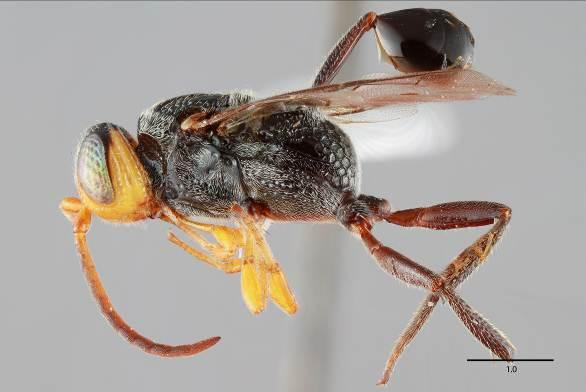
\includegraphics[width=\textwidth]{EvaniidHabitus}
  \caption{Lateral habitus Photo (CC BY 2.0) by \cite{MullinsEtAl2012}}
  \label{fig:evaniid1}
\end{subfigure}
    \hfill
\begin{subfigure}[ht!]{0.45\textwidth}
    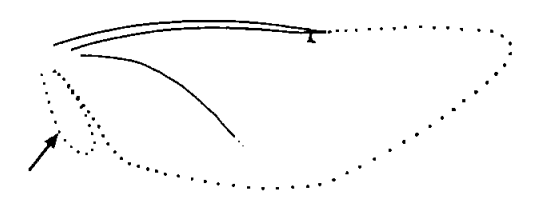
\includegraphics[width=\textwidth]{EvaniidWing}
  \caption{Hind wing \citep[][pg. 510]{goulet1993hymenoptera}}
  \label{fig:evaniid2}
\end{subfigure}
    \caption{Evaniidae}
    \label{fig:evaniid}
\end{figure}

\subsubsection{Megaspilidae}
\begin{itemize}
\item antenna with 12 antennomeres (Figure \ref{fig:megaspilid2})
\item fore wing with no cells enclosed by tubular veins (Figure \ref{fig:megaspilid1})
\item fore wing with only 1 proximal tubular vein on anterior margin
\item pterostigma distinct
\item \textit{protibia with two apical spurs}
\item pronotum is adjacent to tegula in lateral view (compare to families in Chalcidoidea)
\end{itemize}

\begin{figure}[ht!]
  \centering
\begin{subfigure}[ht!]{0.45\textwidth}
    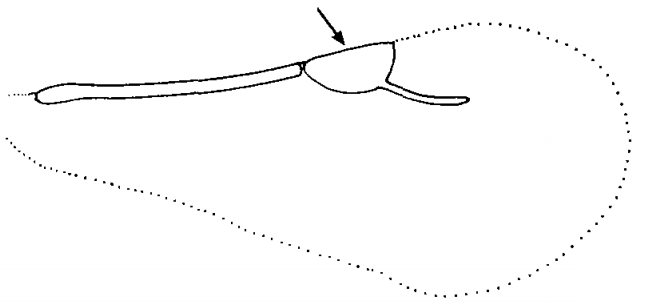
\includegraphics[width=\textwidth]{MegaspilidWing}
  \caption{Fore wing \citep[][pg. 566]{goulet1993hymenoptera}}
  \label{fig:megaspilid1}
\end{subfigure}
    \hfill
\begin{subfigure}[ht!]{0.45\textwidth}
    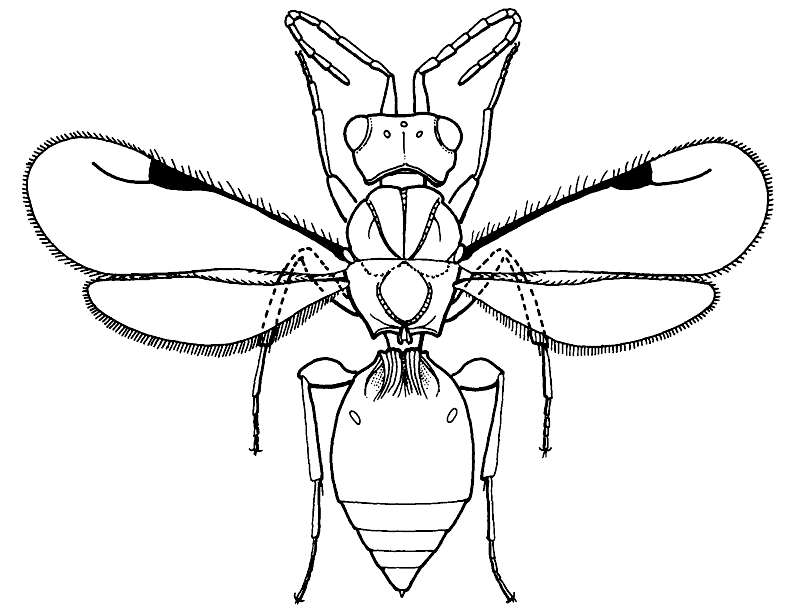
\includegraphics[width=\textwidth]{MegaspilidHabitus}
  \caption{Dorsal habitus \citep[][Fig. 209]{goulet1993hymenoptera}}
  \label{fig:megaspilid2}
\end{subfigure}
    \caption{Megaspilidae}\label{fig:megaspilid}
\end{figure}

\subsubsection{Diapriidae}
\begin{itemize}
\item antenna elbowed
\item antennal shelf present, articulation dorsally distant from clypeus
\item antenna with 11--15 antennomeres
\item fore wing venation variable (sometimes lacking wing cells)
\item usually black or brown, often shiny and smooth in parts
\item petiole tubular
 \end{itemize}

\begin{figure}[ht!]
  \centering
    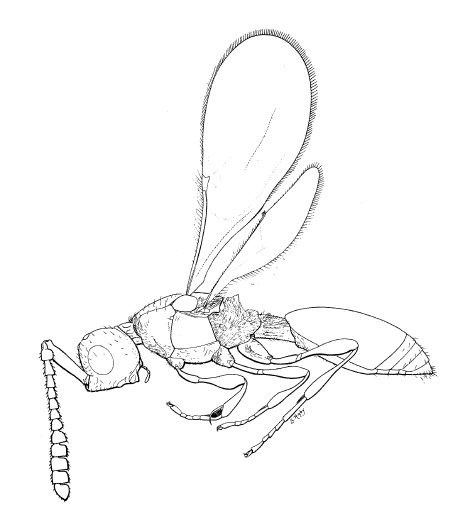
\includegraphics[width=0.45\textwidth]{DiapriidHabitus}
  \caption{Diapriidae habitus \citep[][Fig. 206]{goulet1993hymenoptera}}
  \label{fig:diapriid1}
\end{figure}

\subsubsection{Pelecinidae}
\begin{itemize}
\item relatively large (20--70 mm long)
\item fore wing with one cell enclosed by tubular veins
\item petiole tubular, female abdominal segments elongate, tubular (Figure \ref{fig:pelecinid1})
\end{itemize}

\begin{figure}[ht!]
  \centering
    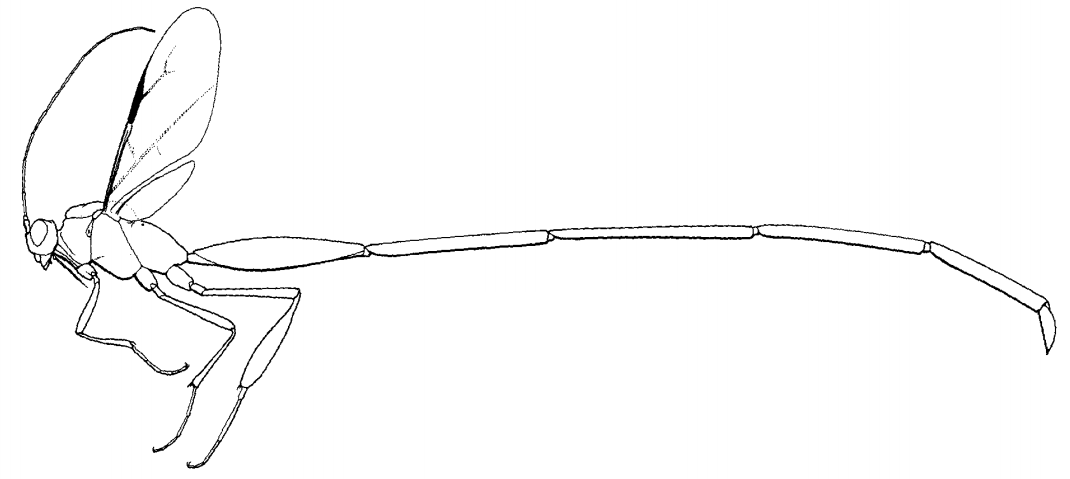
\includegraphics[width=0.75\textwidth]{PelecinidHabitus}
  \caption{Pelecinidae, female habitus. \citep[][Fig. 198]{goulet1993hymenoptera}}
  \label{fig:pelecinid1}
\end{figure}

\subsubsection{Scelionidae}
\begin{itemize}
\item antenna elbowed
\item antennal shelf absent
\item antennal sockets usually close to clypeus
\item fore wing with 3 veins, pterostigma absent (Figure \ref{fig:scelionid1})
\item fore wing without proximal tubular vein on anterior margin
\item antenna usually with 11--12 antennomeres
\item small to very small, usually black or brown
\item pronotum adjacent to tegula
\item petiole not tubular
\item abdomen often flat, with sharp lateral edges
\end{itemize}
\noindent{}These wasps are parasitoids of insect eggs. What do you notice about their body shapes? What do you think is the biological significance?\\

\begin{figure}[ht!]
  \centering
\begin{subfigure}[ht!]{0.45\textwidth}
    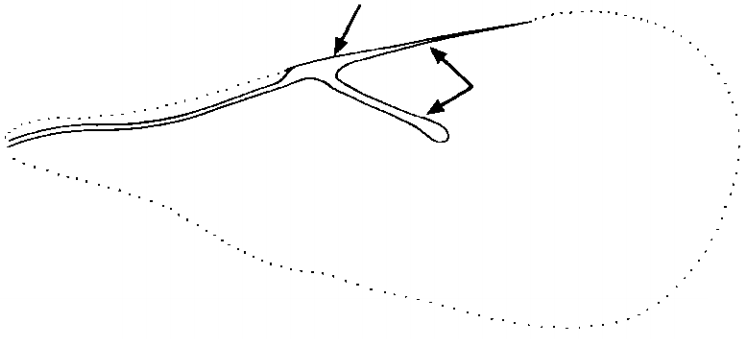
\includegraphics[width=\textwidth]{ScelionidWing}
  \caption{Fore wing \citep[][pg. 560]{goulet1993hymenoptera}}
  \label{fig:scelionid1}
\end{subfigure}
    \hfill
\begin{subfigure}[ht!]{0.45\textwidth}
    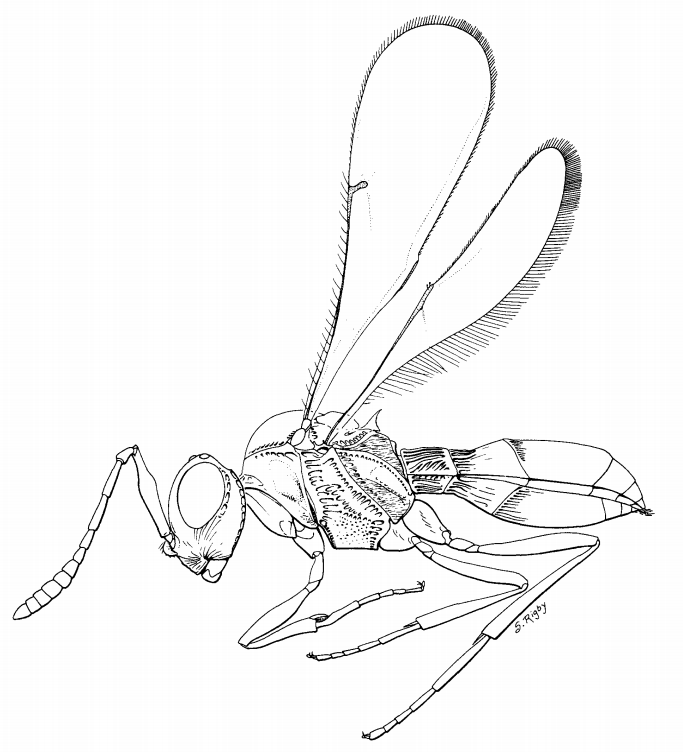
\includegraphics[width=\textwidth]{ScelionidHabitus}
  \caption{Lateral habitus \citep[][Fig. 207]{goulet1993hymenoptera}}
  \label{fig:scelionid2}
\end{subfigure}
    \caption{Scelionidae}\label{fig:scelionids}
\end{figure}

\noindent{}The families below are classified in Cynipoidea, which share the following characteristics:
\begin{itemize}
\item distinctive wing venation: no proximal vein along anterior margin, with well developed marginal cell (R1), no pterostigma
\item pronotum not reaching tegula
\item antenna with 11--16 antennomeres, not elbowed
\item fore wing without proximal tubular vein anteriorly
\item abdomen laterally flattened
\end{itemize}

\subsubsection{Figitidae}
\begin{itemize}
\item fore wing with cell RI 3--4 times as long as wide
\item hind leg with tarsomere 1 not longer than remaining tarsomeres combined
\item petiole of metasoma usually elongate, longer than wide
\item scutellum usually elaborate, with keel or oval elevation
\item if scutellum not elaborate, then 3 abdominal tergites visible or head wider than mesosoma
\end{itemize}

\begin{figure}[ht!]
  \centering
\begin{subfigure}[ht!]{0.45\textwidth}
    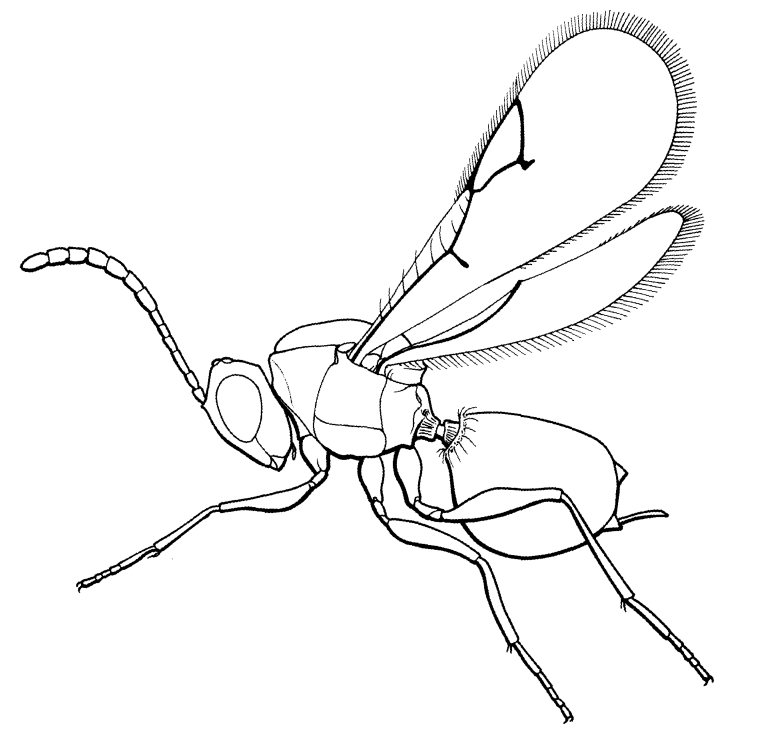
\includegraphics[width=\textwidth]{FigitidHabitus}
  \caption{Figitidae habitus \citep[][Fig. 195]{goulet1993hymenoptera}}
  \label{fig:figid1}
\end{subfigure}
    \hfill
\begin{subfigure}[ht!]{0.42\textwidth}
    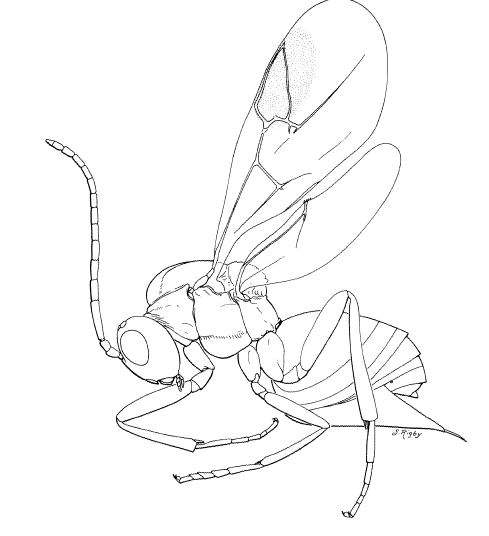
\includegraphics[width=\textwidth]{CynipidHabitus}
  \caption{Cynipidae habitus \citep[][Fig. 197]{goulet1993hymenoptera}}
  \label{fig:cynipid1}
\end{subfigure}
    \caption{Cynipoidea}\label{fig:cynipoids}
\end{figure}

\subsubsection{Cynipidae (gall wasps)}
\begin{itemize}
\item fore wing with cell RI 3--4 times as long as wide
\item hind leg with tarsomere 1 not longer than remaining tarsomeres combined
\item petiole of metasoma hidden or wider than long (Figure \ref{fig:cynipid1})
\item scutellum rounded, not elaborate
\item \textgreater{}3 abdominal tergites visible, head always wider than mesosoma
\end{itemize}

\noindent{}The next families are classified in the super diverse taxon Chalcidoidea. We'll look at five families, but keep in mind there are more than 20 chalcidoid families worldwide, many of wich are quite common in Pennsylvania! They all share the following characteristics, the combination of which separates chalcidoids from other apocritans:
\begin{itemize}
\item antenna elbowed
\item `ring segments' on antenna (short, ringlike sclerites at the base of the flagellum) usually present
\item pronotum not reaching tegula; \textit{i.e.}, a sclerite (prepectus) is present between the pronotum and tegula 
\item fore wing with 3 veins, similar to Scelionidae
\end{itemize}

\subsubsection{Chalcididae (chalcidid wasps)}
\begin{itemize}
\item tarsi 5-segmented
\item hind femora greatly swollen and often toothed, hind tibiae curved to fit femora (Figure \ref{fig:chalcidid})
\item hind coxae much larger than front coxae (Figure \ref{fig:chalcidid})
\item fairly large (for chalcidoids!) 
\item very rarely (if ever) metallic in color
\end{itemize}
\noindent{}What do you think is/are the function(s) of the hind femora in Chalcididae? What makes them so large?

\begin{figure}[ht!]
  \centering
\begin{subfigure}[ht!]{0.45\textwidth}
    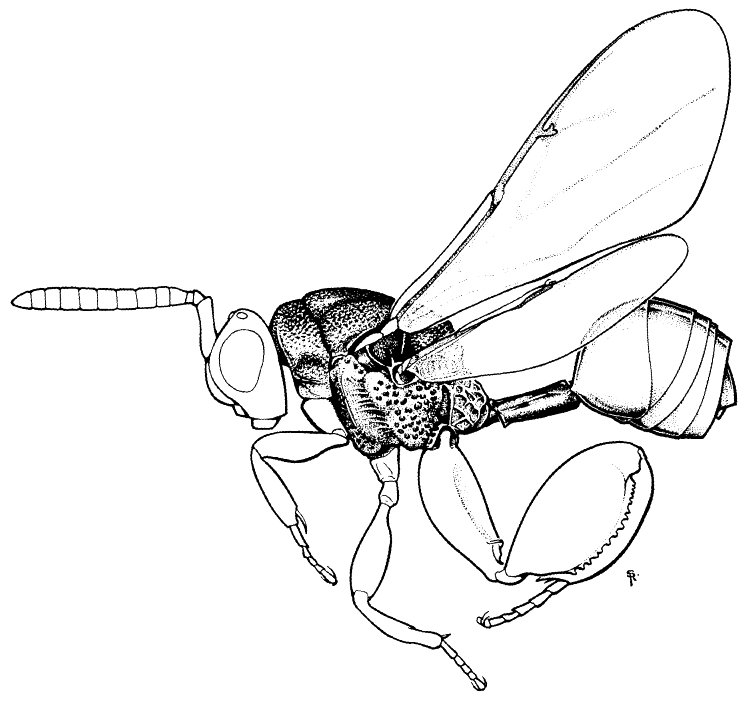
\includegraphics[width=\textwidth]{ChalcididHabitus}
  \caption{Chalcididae lateral habitus \citep[][Fig. 212]{goulet1993hymenoptera}}
  \label{fig:chalcidid}
\end{subfigure}
    \hfill
\begin{subfigure}[ht!]{0.45\textwidth}
    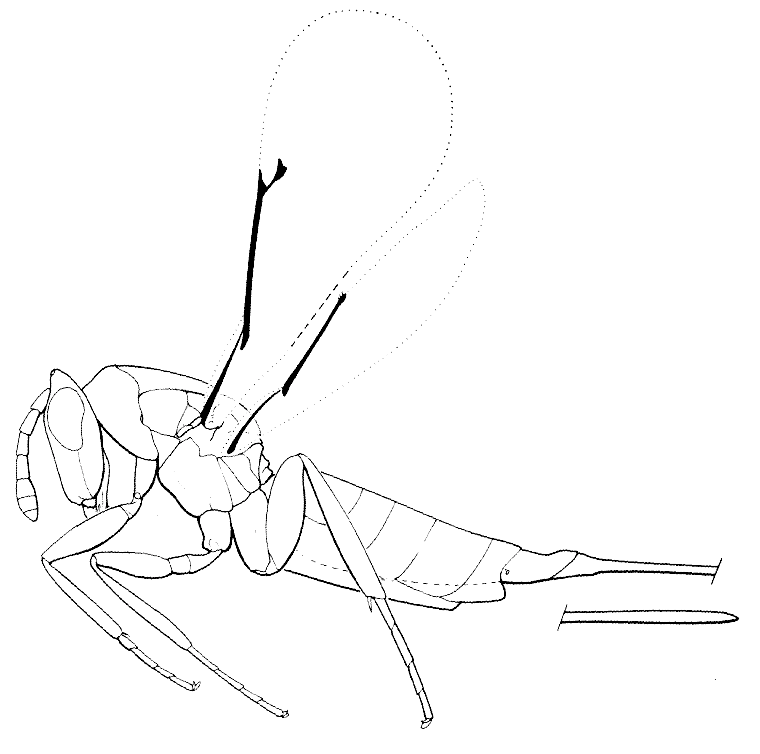
\includegraphics[width=\textwidth]{EulophidHabitus}
  \caption{Eulophidae habitus \citep[][Fig. 228]{goulet1993hymenoptera}}
  \label{fig:eulophid}
\end{subfigure}
\label{fig:xxxxxx}
\end{figure}

\subsubsection{Eulophidae (eulophid wasps)}
\begin{itemize}
\item antennal funicle with 4 or fewer antennomeres
\item tarsi 4-segmented (Figure \ref{fig:eulophid})
\item apical spur of front tibiae short and straight
\item small, often black, brown, or blue
\end{itemize}

\subsubsection{Encyrtidae}
\begin{itemize}
\item mesopleuron strongly convex, without grooves (Figure \ref{fig:encyrt1})
\item tarsi usually 5-segmented
\item if tarsi 4-segmented, funicle with 5+ antennomeres
\item apical spur of middle tibiae large
\item usually rather stout-bodied and very small
\item cerci distinctly anterior to apical abdominal margin (Figure \ref{fig:encyrt2})
\end{itemize}

\begin{figure}[ht!]
  \centering
\begin{subfigure}[ht!]{0.55\textwidth}
    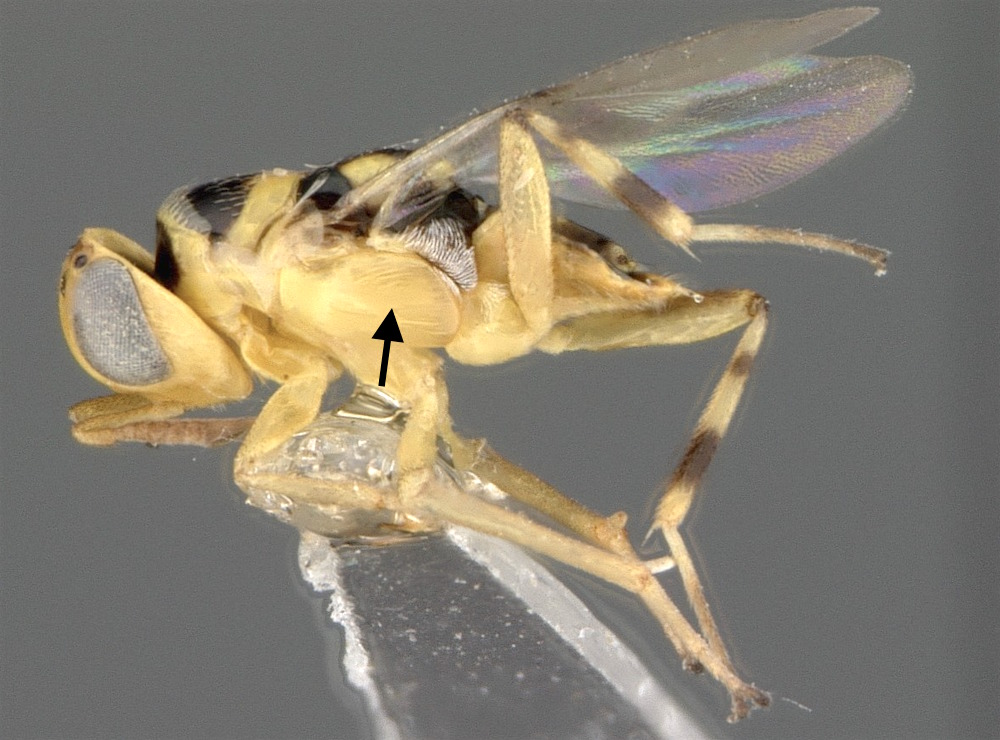
\includegraphics[width=\textwidth]{EncyrtidHabitus}
  \caption{Habitus. Photo CC0 by Michael Gates \url{http://morphbank.net/?id=228742}}
  \label{fig:encyrt1}
\end{subfigure}
    \hfill
\begin{subfigure}[ht!]{0.35\textwidth}
    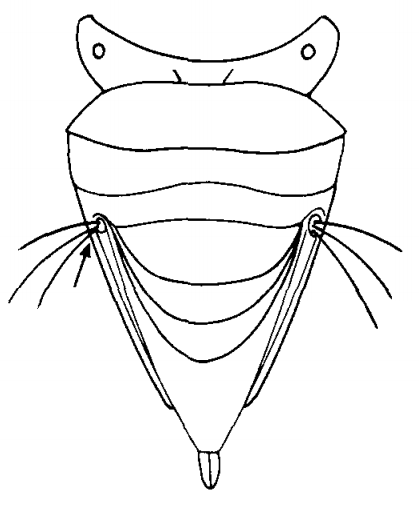
\includegraphics[width=\textwidth]{EncyrtidMetasoma}
  \caption{Metasoma in dorsal view \citep[][pg. 581]{goulet1993hymenoptera}}
  \label{fig:encyrt2}
\end{subfigure}
    \caption{Encyrtidae}\label{fig:encyrt}
\end{figure}

\subsubsection{Mymaridae (fairyflies)}
\begin{itemize}
\item body typically very small (these wasps are parasitoids of insect eggs)
\item head with H-shaped complex bar-like structures on face (trabeculae)
\item wings fringed
\item hind wing stalked proximally
\end{itemize}

\begin{figure}[ht!]
  \centering
\begin{subfigure}[ht!]{0.5\textwidth}
    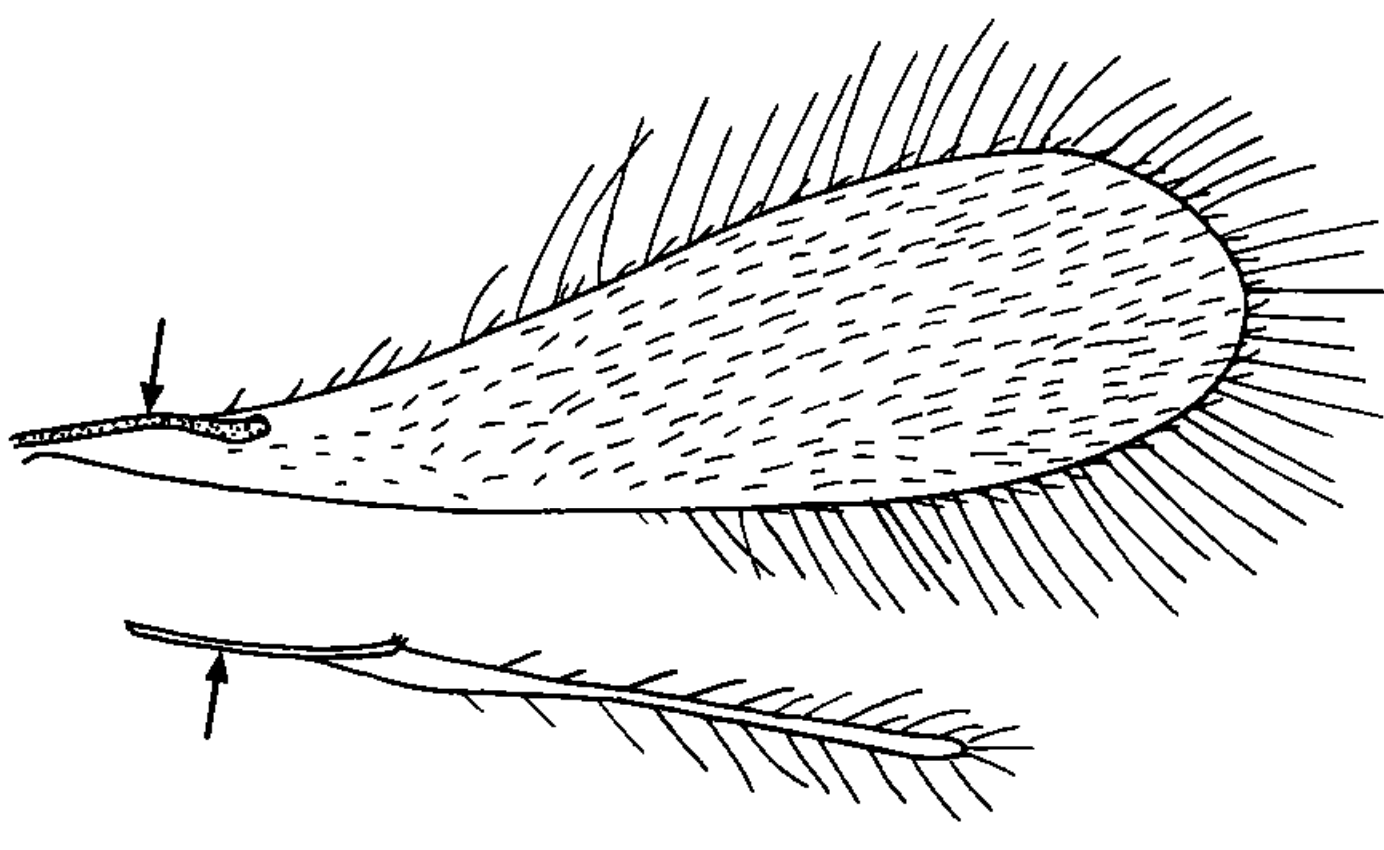
\includegraphics[width=\textwidth]{MymaridWings}
  \caption{Wings}
  \label{fig:mymarid1}
\end{subfigure}
    \qquad
\begin{subfigure}[ht!]{0.28\textwidth}
    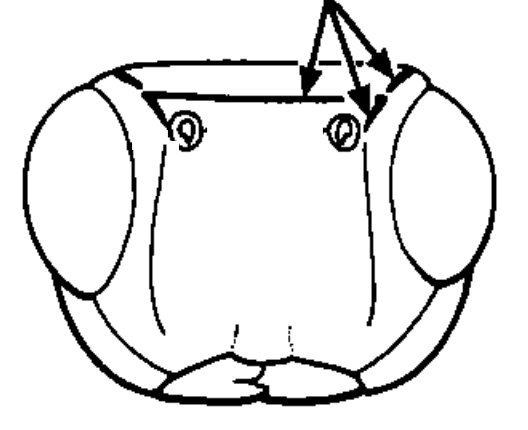
\includegraphics[width=\textwidth]{MymaridHead}
  \caption{Head in anterior view}
  \label{fig:mymarid2}
\end{subfigure}
    \caption{Mymaridae \citep[][pg. 87]{goulet1993hymenoptera}}\label{fig:mymarids}
\end{figure}

\paragraph*{Aculeata} In Aculeata, the egg does not enter the ovipositor assembly prior to deposition but rather leaves the metasoma anterior to the ovipositor. The ovipositor functions only to inject venom gland products (\textit{i.e.}, venom). Besides the structure of the ovipositor, the monophyly of Aculeata is supported mostly by indistinct internal characters (\textit{e.g.}, the shape, pattern and presence/absence of thoracic muscles). The only distinct synapomorphy of the infraorder is the presence of the supramesopleural sclerite (sms), that partially obscures the second thoracic spiracle. (Caveat: The sms is absent from a few Aculeata and \textit{present} in some non-aculeates, like Evaniidae and Trigonalidae.)

Besides the above-mentioned synapomorphies, Aculeata can be superficially characterized by their well-developed wing venation (but see some ``Chrysidoidea''), distinct wasp waist (unlike sawflies), well sclerotized metasomal sternites (unlike most Ichneumonoidea), having fewer than 11 flagellomeres (numerous Ichneumonoidea have more than 11 flagellomeres), and convex, almost bulbous metasoma.

Traditionally the infraorder is subdivided into three superfamilies: Chrysidoidea, Apoidea, and Vespoidea. Only the monophyly of Apoidea is supported in the latest phylogenetic analyses.

\subsubsection{Bethylidae}
\begin{itemize}
\item body usually weakly sculptured and brown or black (not typically metallic)
\item head usually prognathous (Figure \ref{fig:bethylid1})
\item antenna with 11 (rarely 10 or 8) flagellomeres
\item pronotum with anterior flange, propleuron thus concealed in dorsal view 
\item distal venation of wing reduced
\item metasoma with 6 or 7 exposed terga
\end{itemize}

\begin{figure}[ht!]
  \centering
\begin{subfigure}[ht!]{0.28\textwidth}
    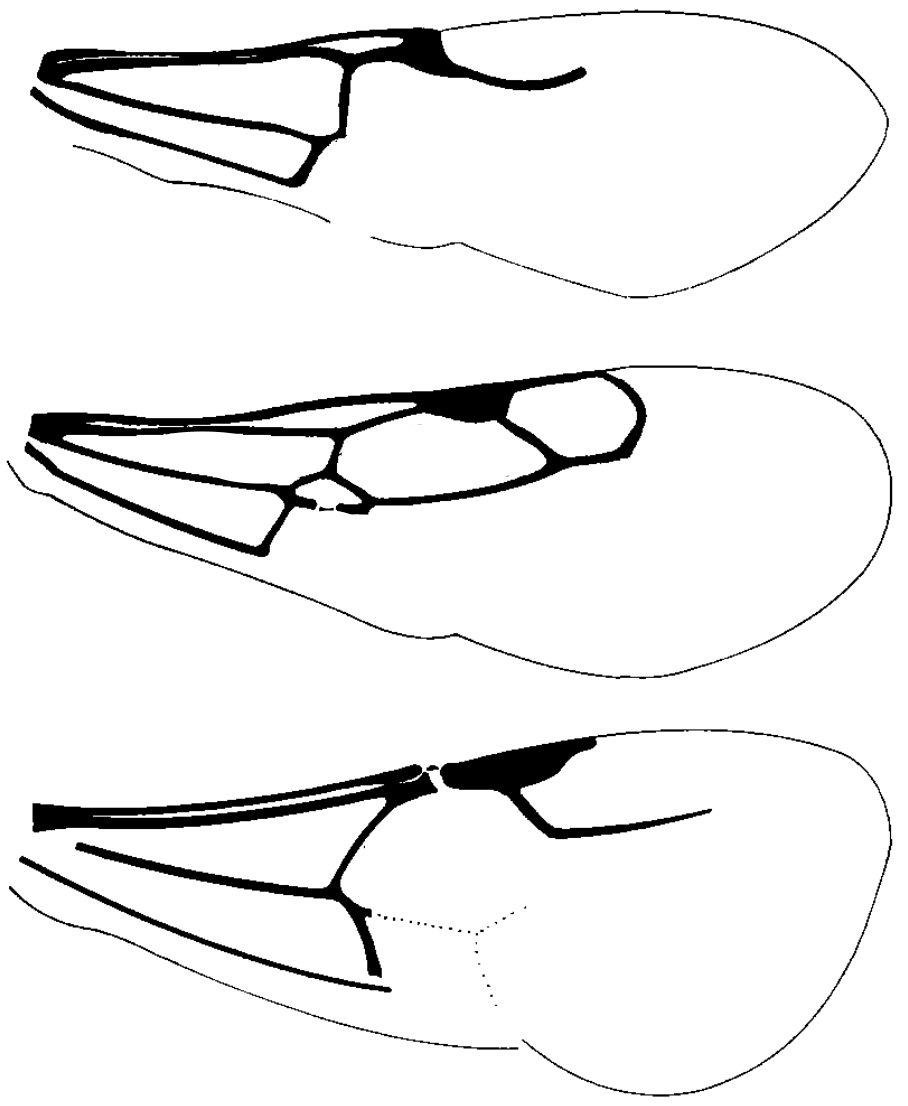
\includegraphics[width=\textwidth]{BethylidWings}
  \caption{Fore wings \citep[][pg. 134]{goulet1993hymenoptera}}
  \label{fig:bethylid1}
\end{subfigure}
    \qquad
\begin{subfigure}[ht!]{0.35\textwidth}
    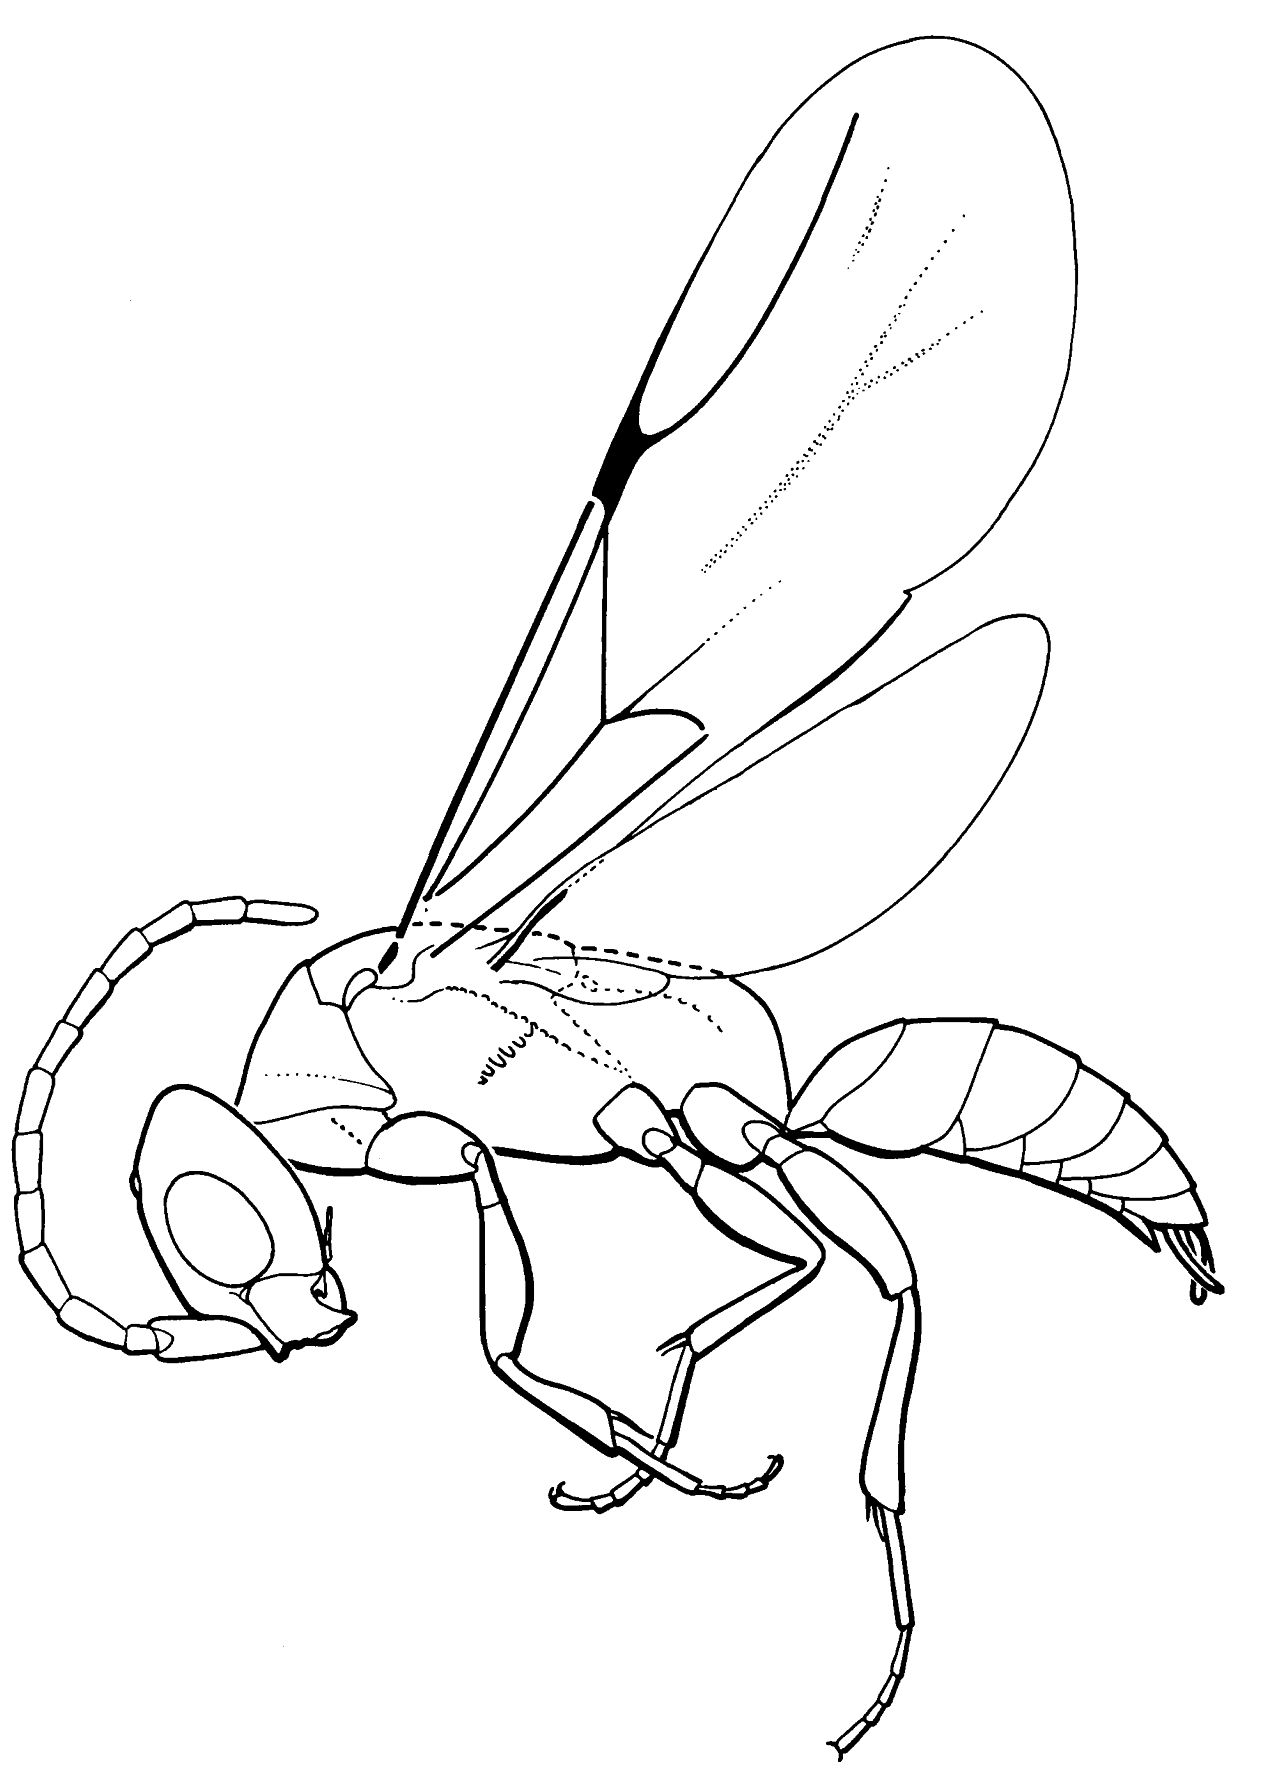
\includegraphics[width=\textwidth]{BethylidHabitus}
  \caption{Habitus \citep[][Fig. 37]{goulet1993hymenoptera}}
  \label{fig:bethylid2}
\end{subfigure}
    \caption{Bethylidae}\label{fig:bethylids}
\end{figure}

\subsubsection{Chrysididae (cuckoo wasps)}
\begin{itemize}
\item head typically hypognathous 
\item antenna with 11 flagellomeres
\item pronotum with anterior flange, thus propleuron concealed in dorsal view 
\item pronotum with posterolateral apex usually well separated from tegula but sometimes touching 
\item metasoma usually with 5 or fewer exposed terga; strongly concave ventrally (Figure \ref{fig:chrysididae})
\item usually strongly sculptured  
\item usually metallic (Figure \ref{fig:chrysid1})
\end{itemize}

\begin{figure}[ht!]
    \centering
    \begin{subfigure}[ht!]{0.42\textwidth}
        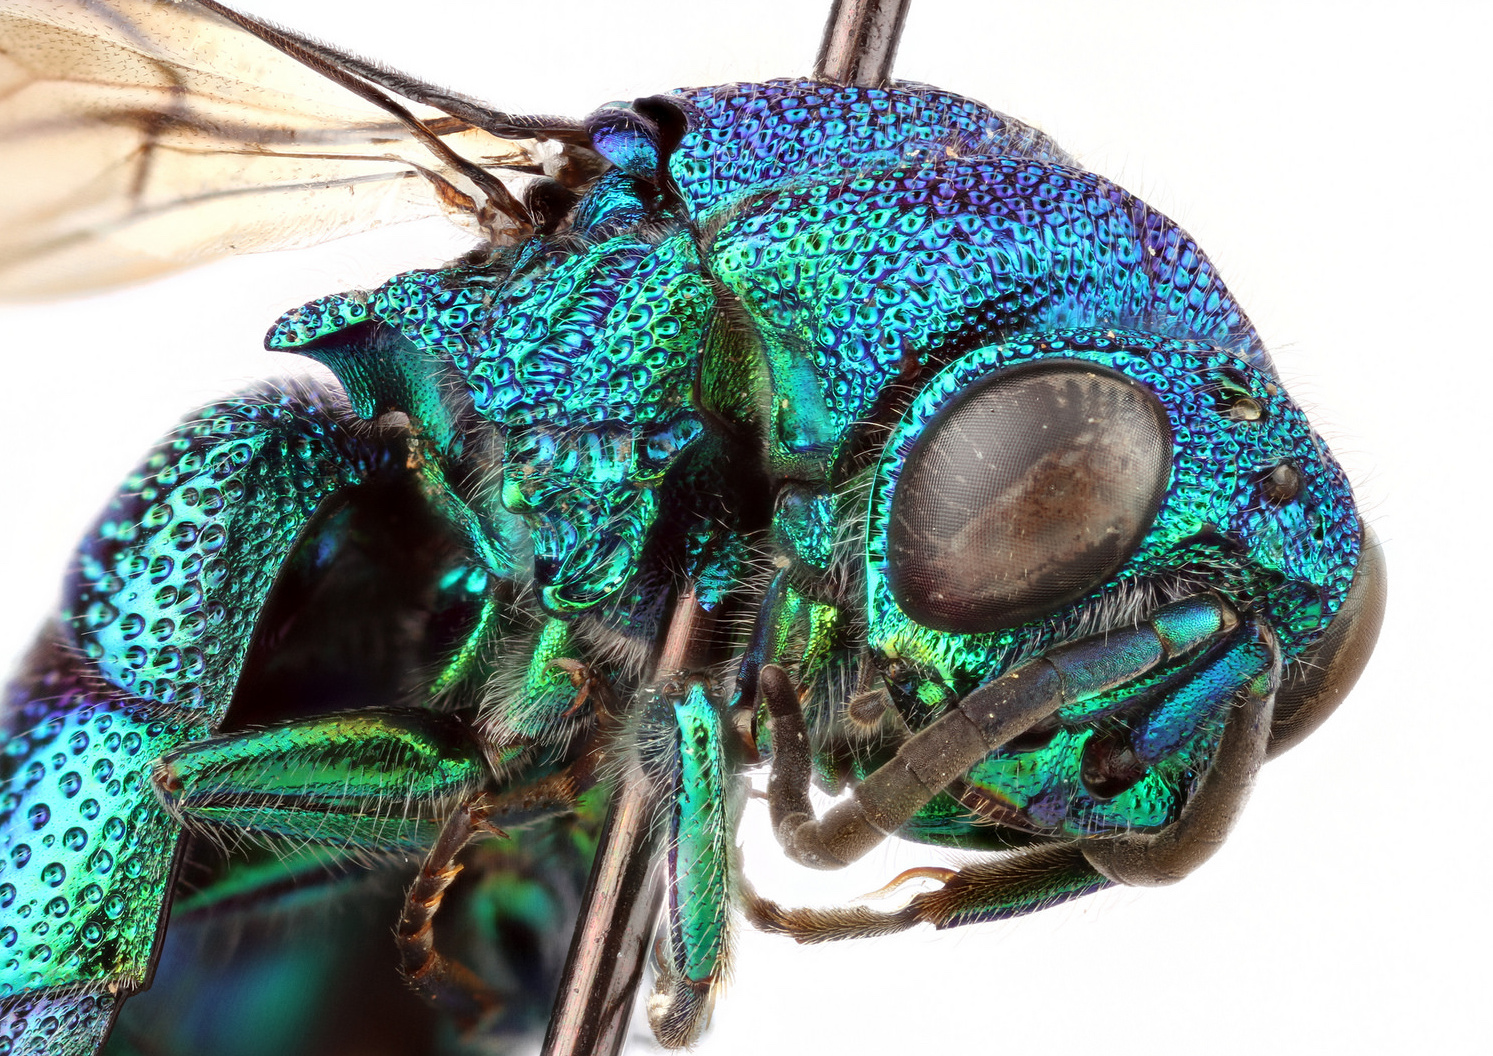
\includegraphics[width=\textwidth]{ChrysididColor}
        \caption{Habitus. Photo CC0 by James Marchment \url{https://flic.kr/p/DciZEn}}
        \label{fig:chrysid1}
    \end{subfigure}
    \qquad
    \begin{subfigure}[ht!]{0.39\textwidth}
        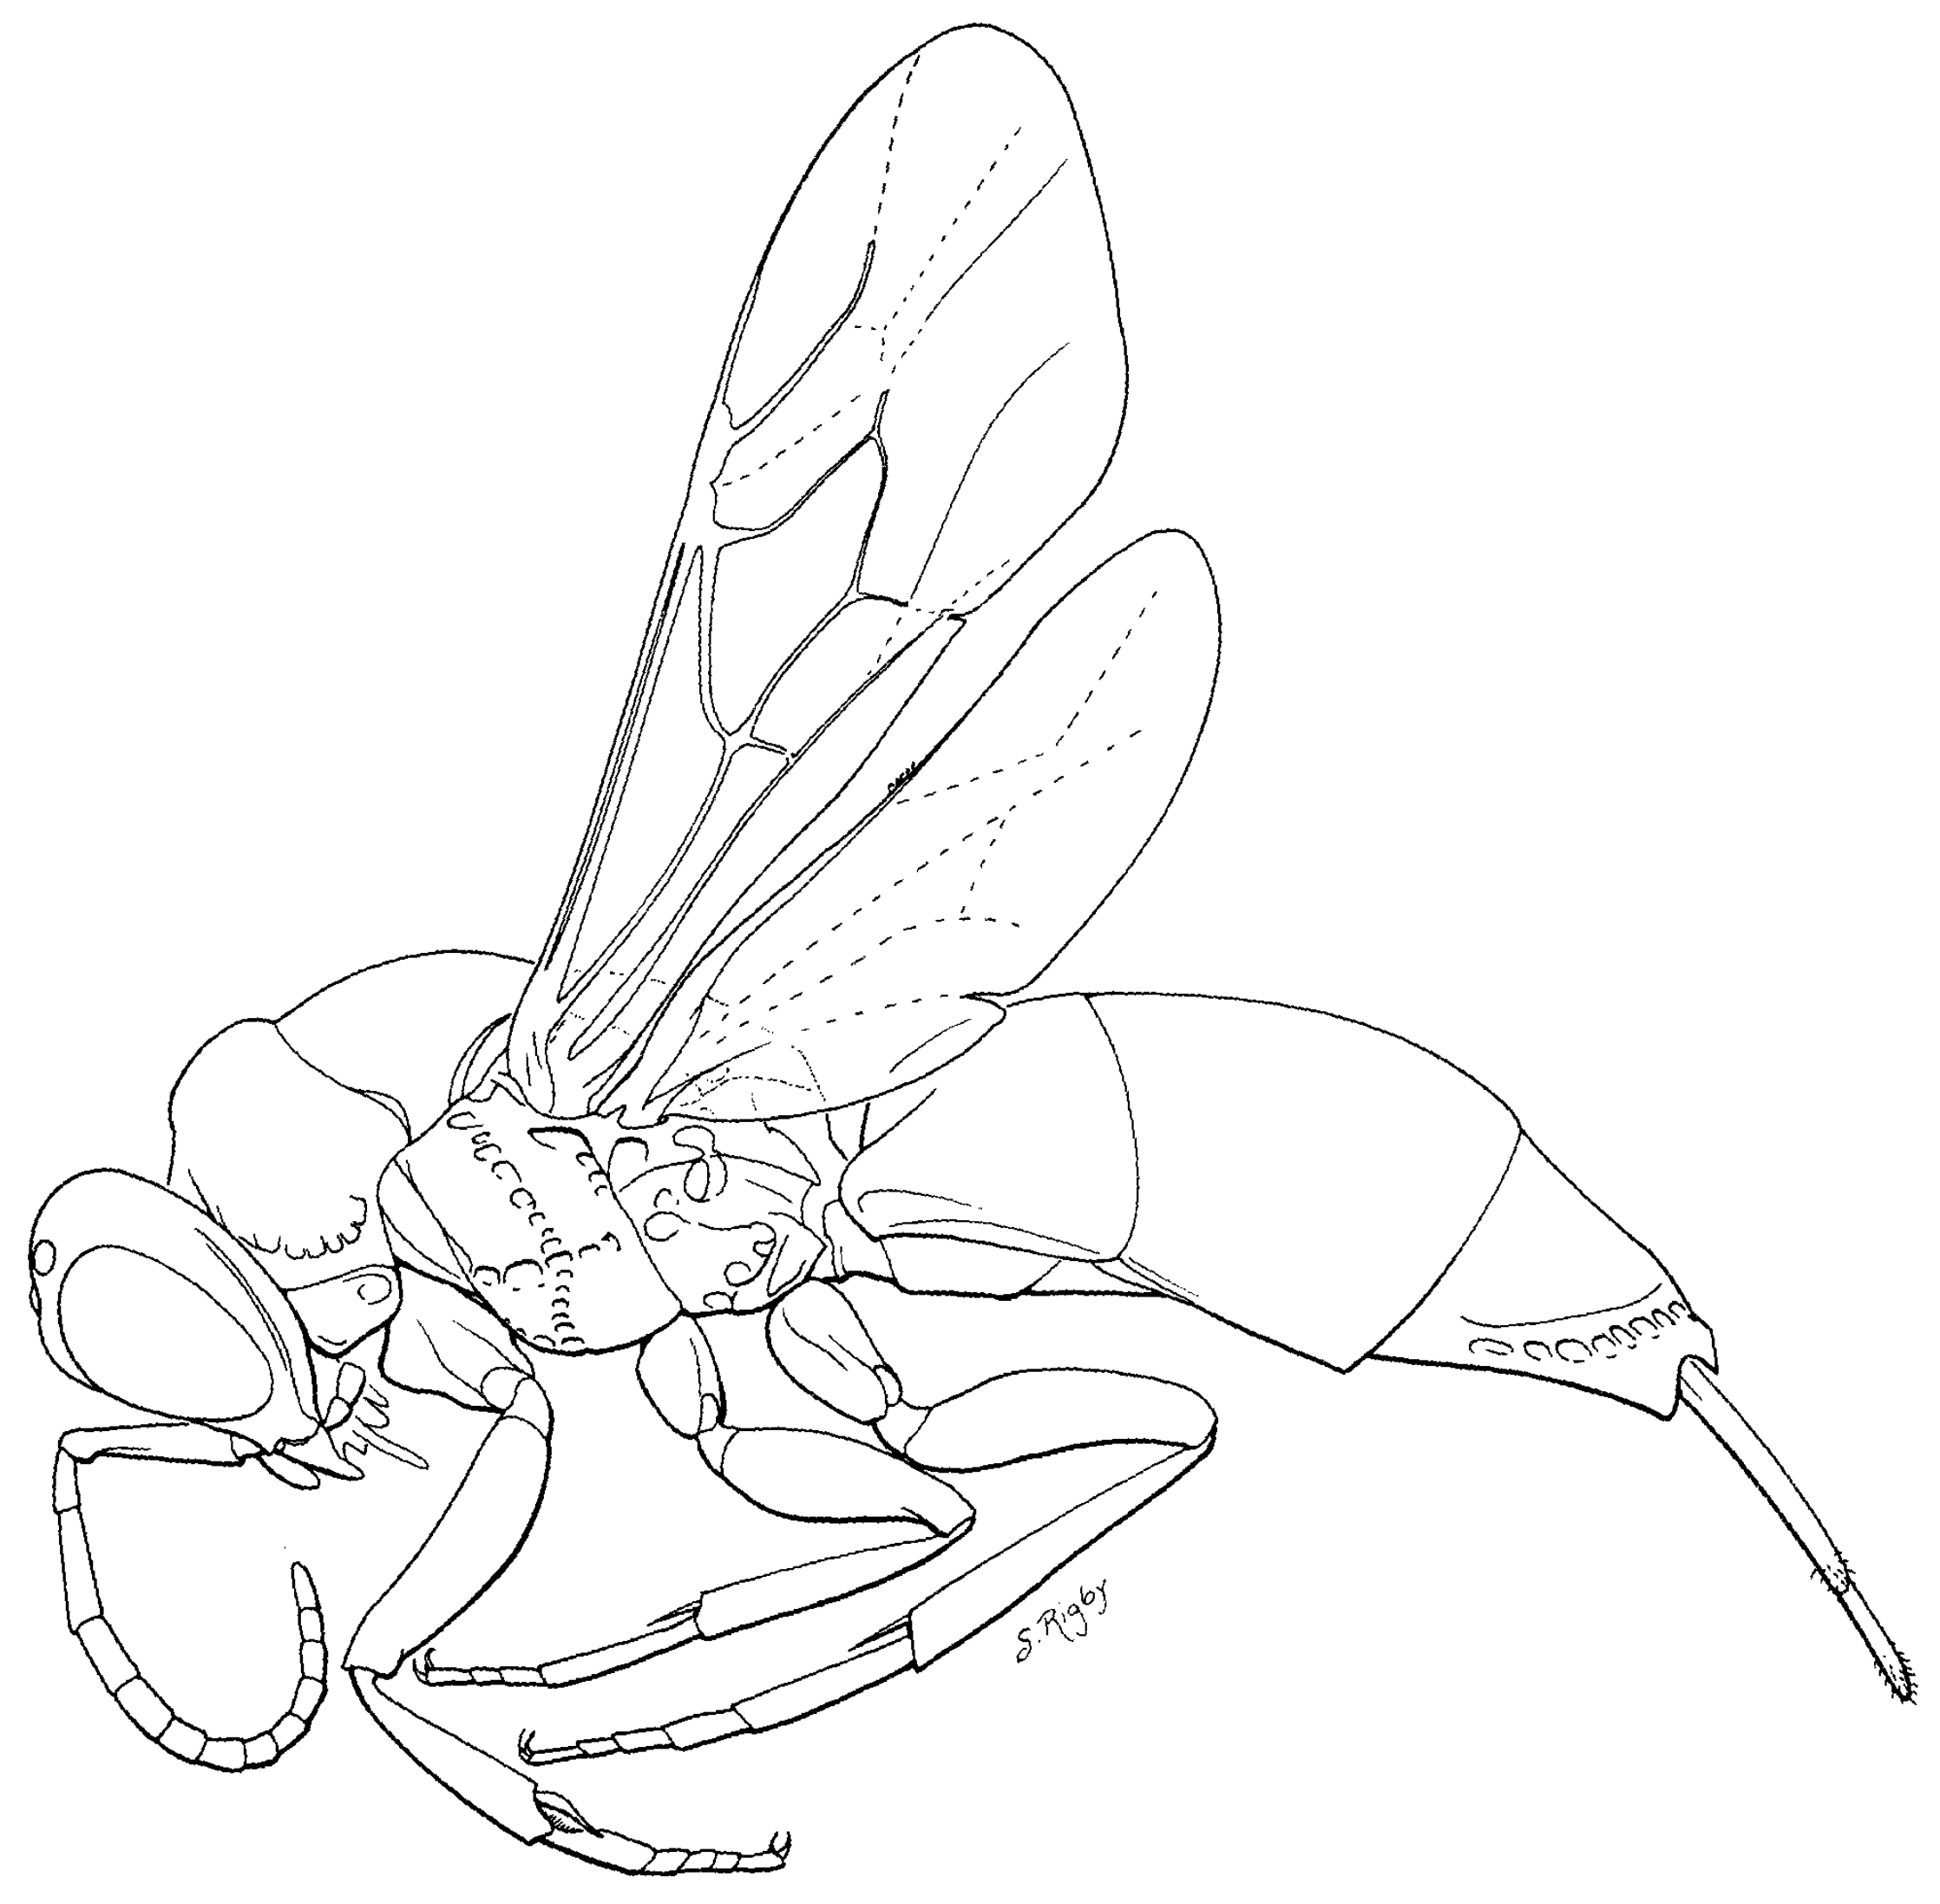
\includegraphics[width=\textwidth]{ChrysididHabitus}
        \caption{Habitus \citep[][Fig. 42]{goulet1993hymenoptera}}
        \label{fig:chrysid2}
    \end{subfigure}
    \caption{Chrysididae}\label{fig:chrysididae}
\end{figure}
\FloatBarrier

\noindent{}The next six families are usually classified in Vespoidea, a taxon comprising 2--11 extant families, depending on whom you ask. Many species are parasitoids, but we're starting to see some that are predators (Vespidae), even pollen gatherers (Vespidae: Masarinae), or with broadly diverse diets (Formicidae). And many species are highly eusocial (many Vespidae, all Formicidae). 

\subsubsection{Tiphiidae}
\begin{itemize}
\item eye not usually ``notched'', like we see in Vespidae
\item mesosternum with laminate expansions on each side of midline covering bases of contiguous mesocoxae, the expansions rarely reduced to small teeth
\item hind wing with deeply separated (jugal) lobe (Figure \ref{fig:tiphiid2})
\item female usually with mesotibia and metatibia stout and spiny
\item metasomal segment 1 without a true node (like we see in Formicidae), although sometimes approaching it
\item male metasomal sternum 8 (hypopygium) usually forming a single strong acute, upcurved hook, the hypopygium sometimes simple or with 2--5 spines, and usually entirely exposed (Figure \ref{fig:tiphiidae})
\end{itemize}

\begin{figure}[ht!]
    \centering
    \begin{subfigure}[ht!]{0.4\textwidth}
        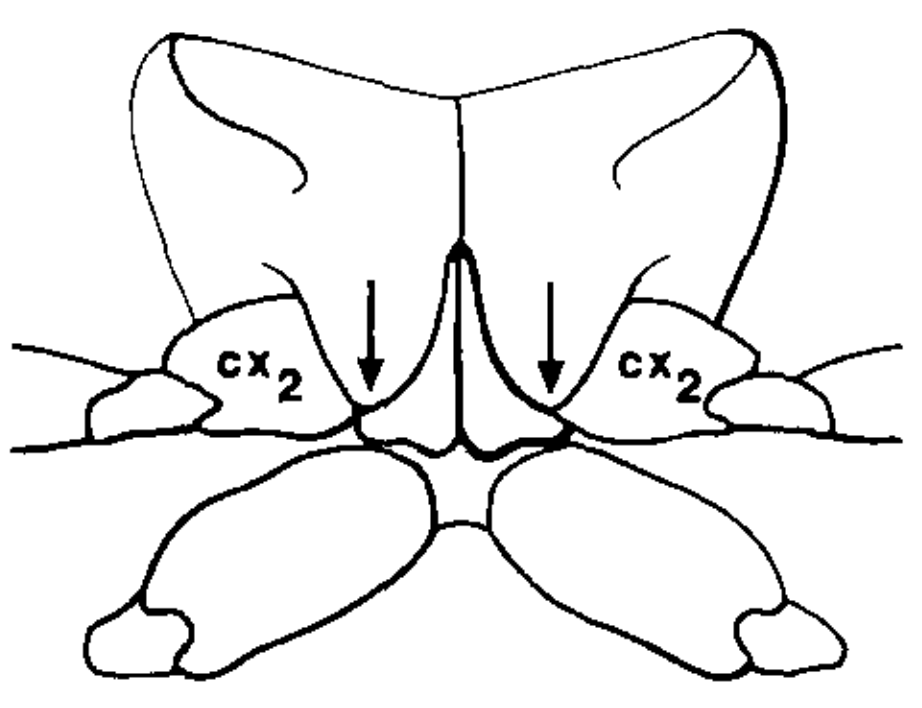
\includegraphics[width=\textwidth]{TiphiidMesosoma}
        \caption{Mesosoma in venral view \citep[][pg. 163]{goulet1993hymenoptera}; cx2 = mesocoxa}
        \label{fig:tiphiid1}
    \end{subfigure}
    \qquad
    \begin{subfigure}[ht!]{0.45\textwidth}
        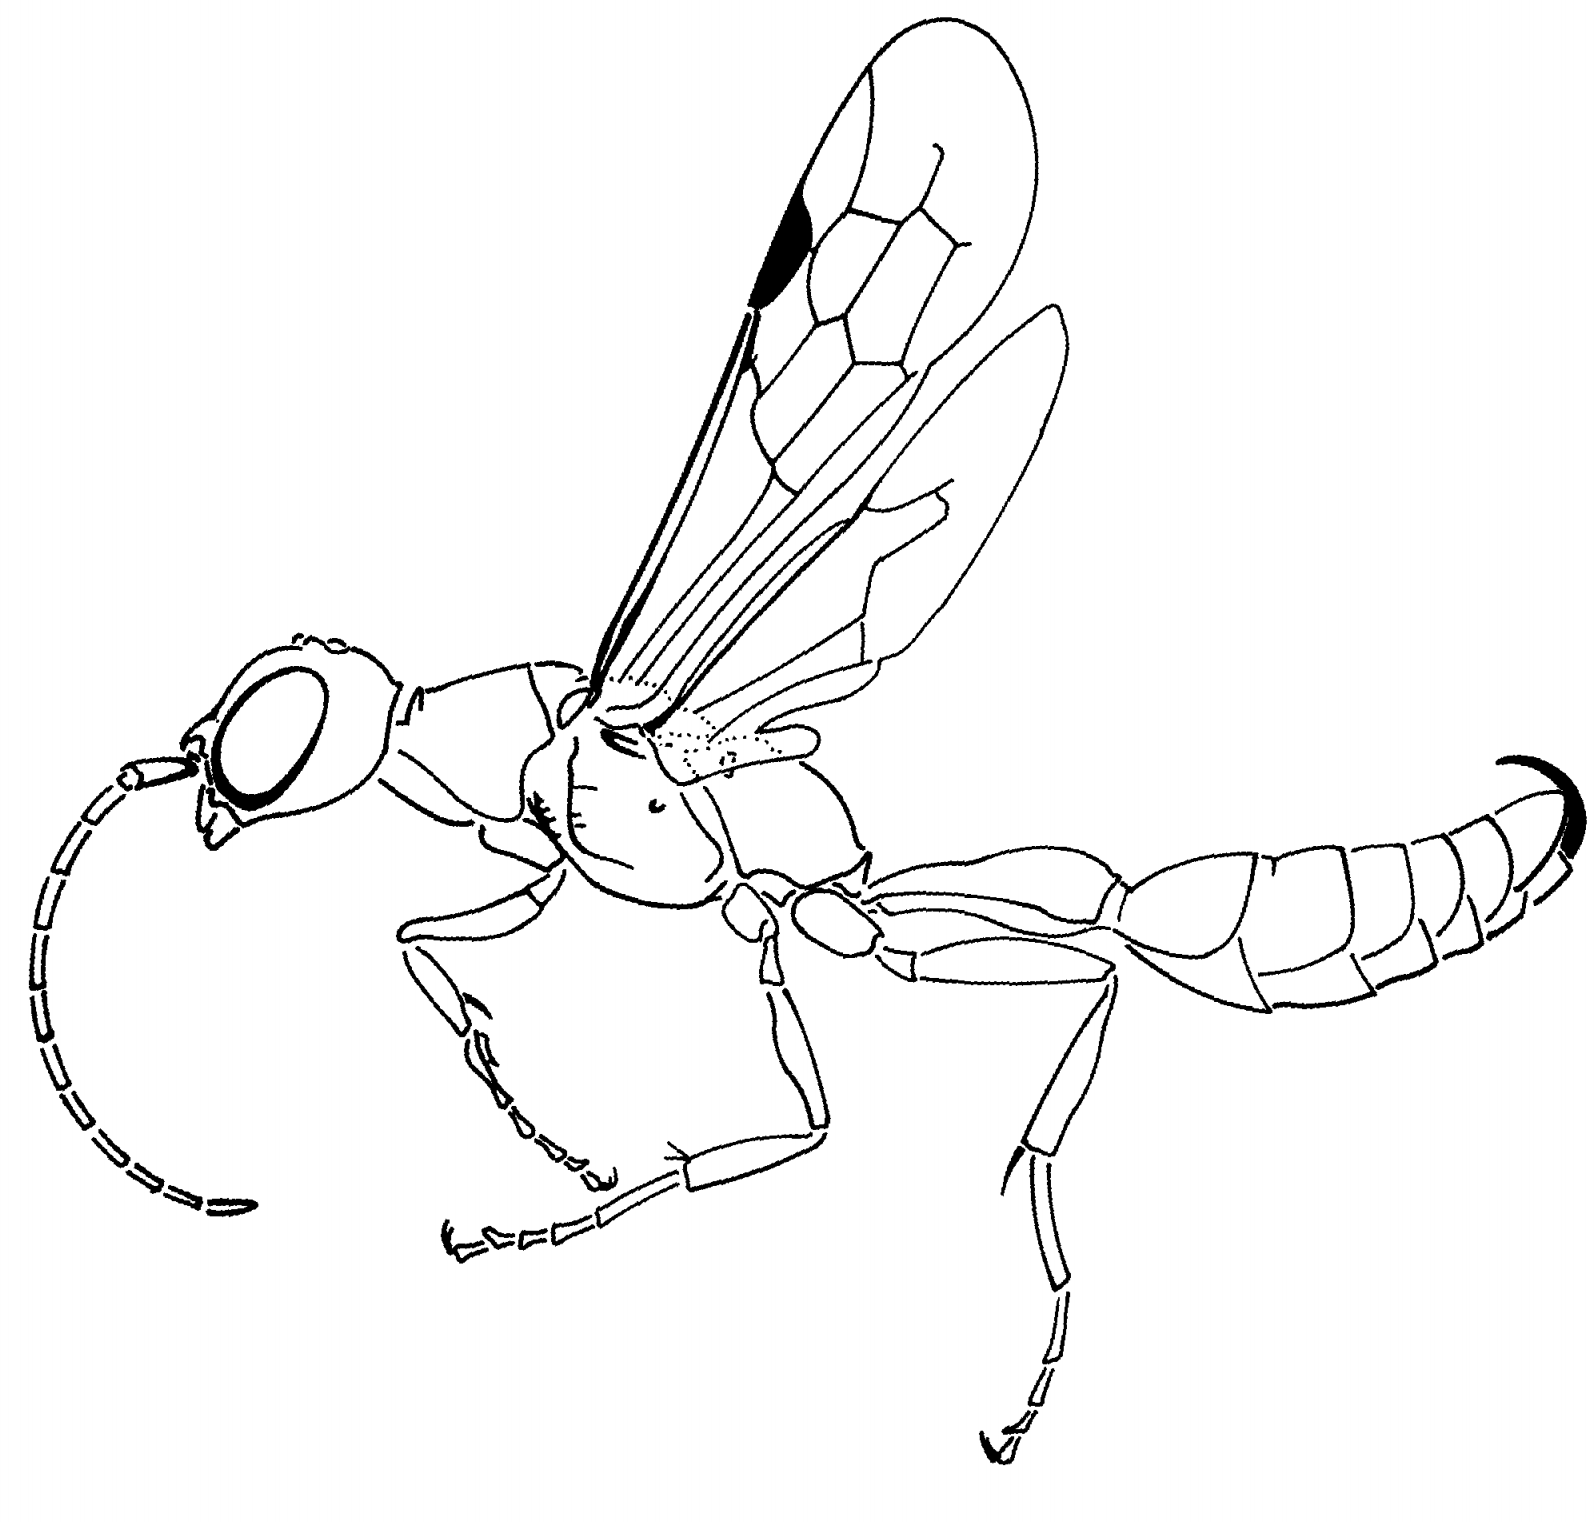
\includegraphics[width=\textwidth]{TiphiidHabitus}
        \caption{Habitus \citep[][Fig. 49]{goulet1993hymenoptera}}
        \label{fig:tiphiid2}
    \end{subfigure}
    \caption{Tiphiidae}\label{fig:tiphiidae}
\end{figure}

\subsubsection{Mutillidae (velvet ants)}
\begin{itemize}
\item metasomal segment 1 without a true node
\item metasomal segment 2 usually with longitudinal felt line or with felted pit on tergum and/or sternum (but sometimes without)
\item female almost always apterous (Figure \ref{fig:mutillid1})
\item apterous forms with pronotum usually fused to mesothorax and mesonotum to metanotum-propodeum complex
\item usually very furry and often colorful or brownish and quite ``bristly'' 
\item body often very hard and difficult to pin
\end{itemize}
Why are velvet ants typically brightly colored? Keep in mind that their stings are quite long (and painful!). Based on their lack of wings (in females, at least) and the \textit{very} heavily sclerotized bodies what would you hypothesize about their life histories?

\begin{figure}[ht!]
    \centering
    \begin{subfigure}[ht!]{0.45\textwidth}
        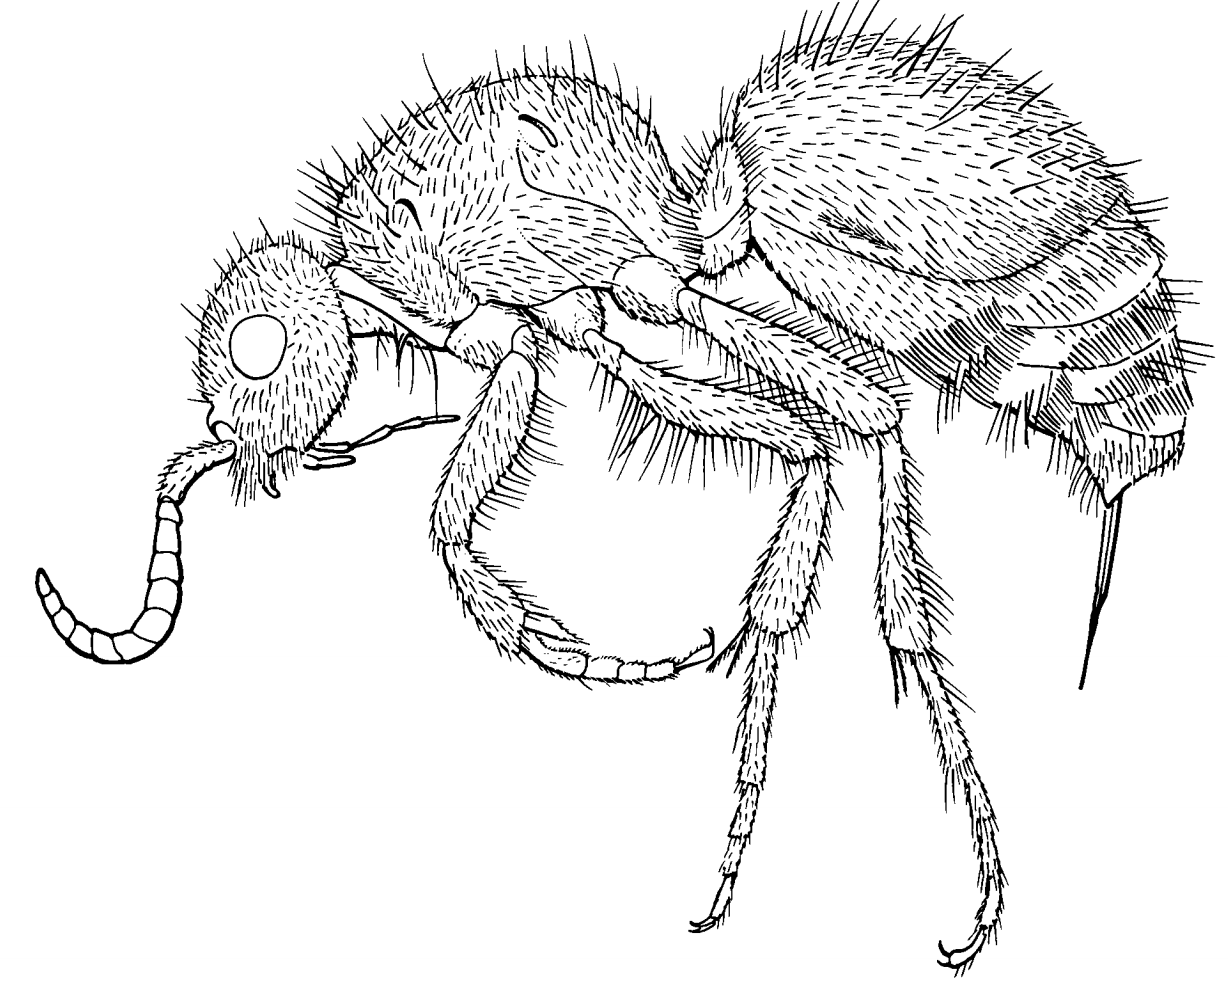
\includegraphics[width=\textwidth]{MutillidHabitus}
        \caption{Female habitus \citep[][Fig. 63]{goulet1993hymenoptera}}
        \label{fig:mutillid1}
    \end{subfigure}
    \qquad
    \begin{subfigure}[ht!]{0.45\textwidth}
        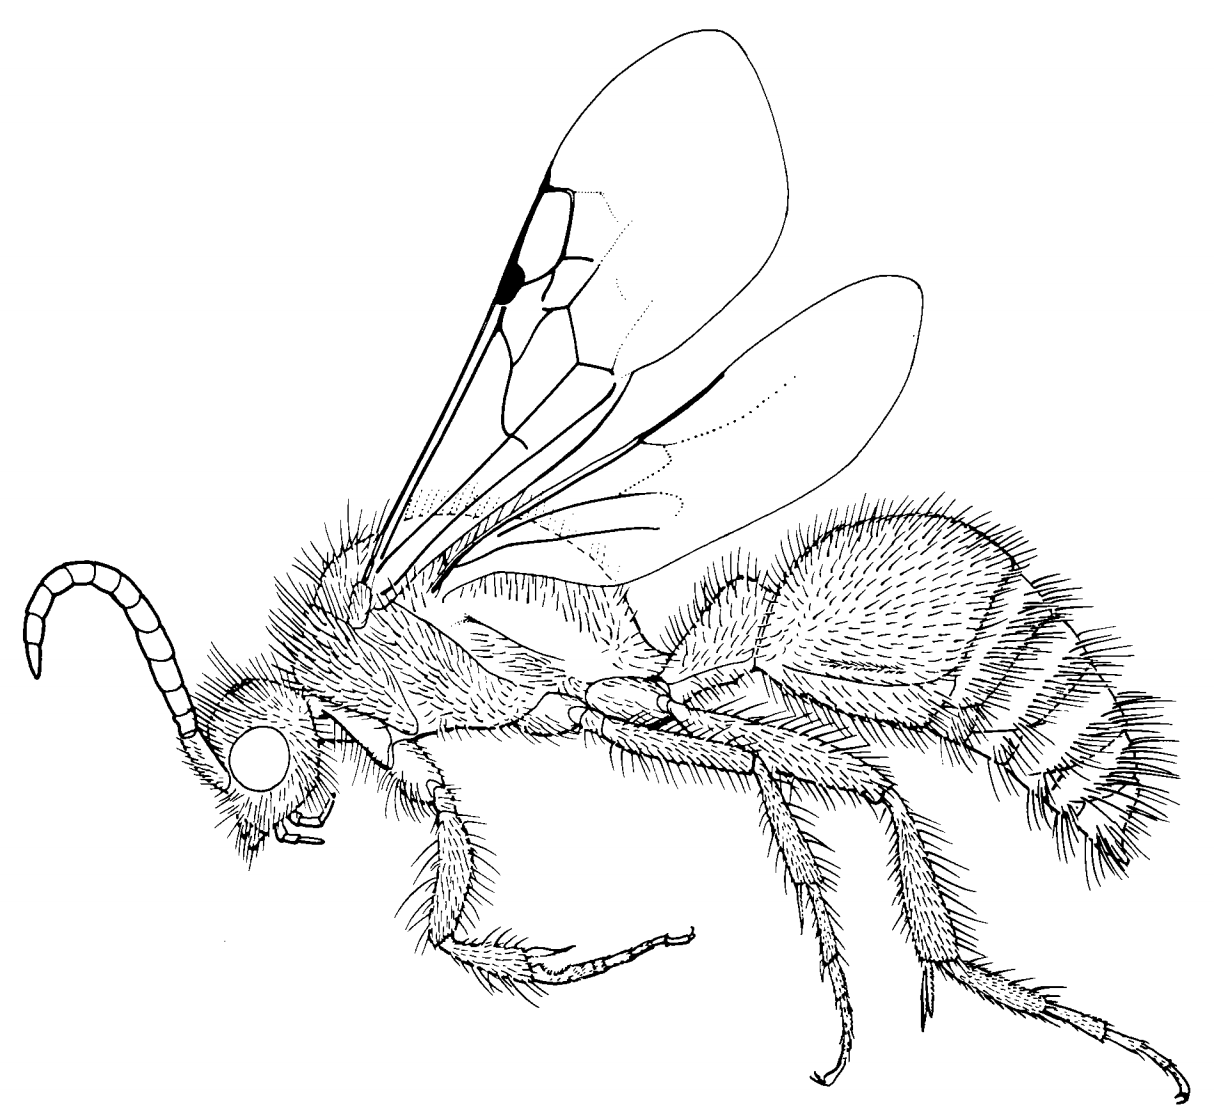
\includegraphics[width=\textwidth]{MaleMutillidHabitus}
        \caption{Male habitus \citep[][Fig. 64]{goulet1993hymenoptera}}
        \label{fig:mutillid2}
    \end{subfigure}
    \caption{Mutillidae}\label{fig:mutillids}
\end{figure}

\subsubsection{Formicidae (ants)}
\begin{itemize}
\item metapleural gland present (in most species), its opening usually distinct
\item posterior (inner) spur of metatibia modified as a calcar 
\item reproductive forms usually macropterous, sterile female apterous 
\item apterous form with with pronotum usually freely articulating but sometimes fused with mesothorax
\item mesonotum and metathorax-propodeum complex usually fused (Figure \ref{fig:formicid1}
\item metasoma petiolate 
\item metasomal segment 1 usually strongly constricted at each end, forming a true node
\item metasomal sternum 1 separated from sternum 2 by a deep constriction
\end{itemize}
Compare apterous specimens to those with wings (alates, or reproductives). Do you see differences in their mesosomal morphology? \\

\noindent{}Do you see any morphological evidence that these insects, ants, are highly eusocial? Remember the three main conditions of eusociality ...\\

\begin{figure}[ht!]
    \centering
    \begin{subfigure}[ht!]{0.42\textwidth}
        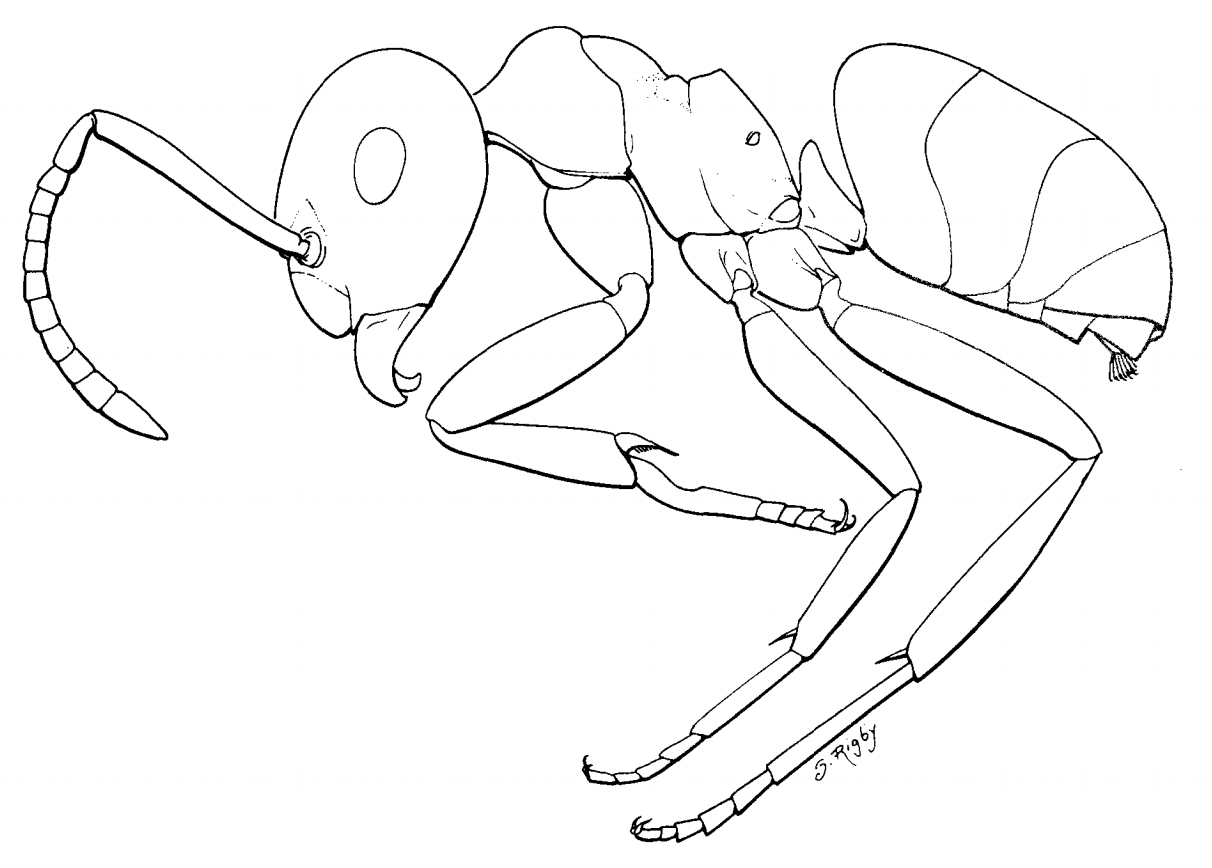
\includegraphics[width=\textwidth]{FemaleFormicidHabitus}
        \caption{Female habitus \citep[][Fig. 91]{goulet1993hymenoptera}}
        \label{fig:formicid1}
    \end{subfigure}
    \qquad
    \begin{subfigure}[ht!]{0.35\textwidth}
        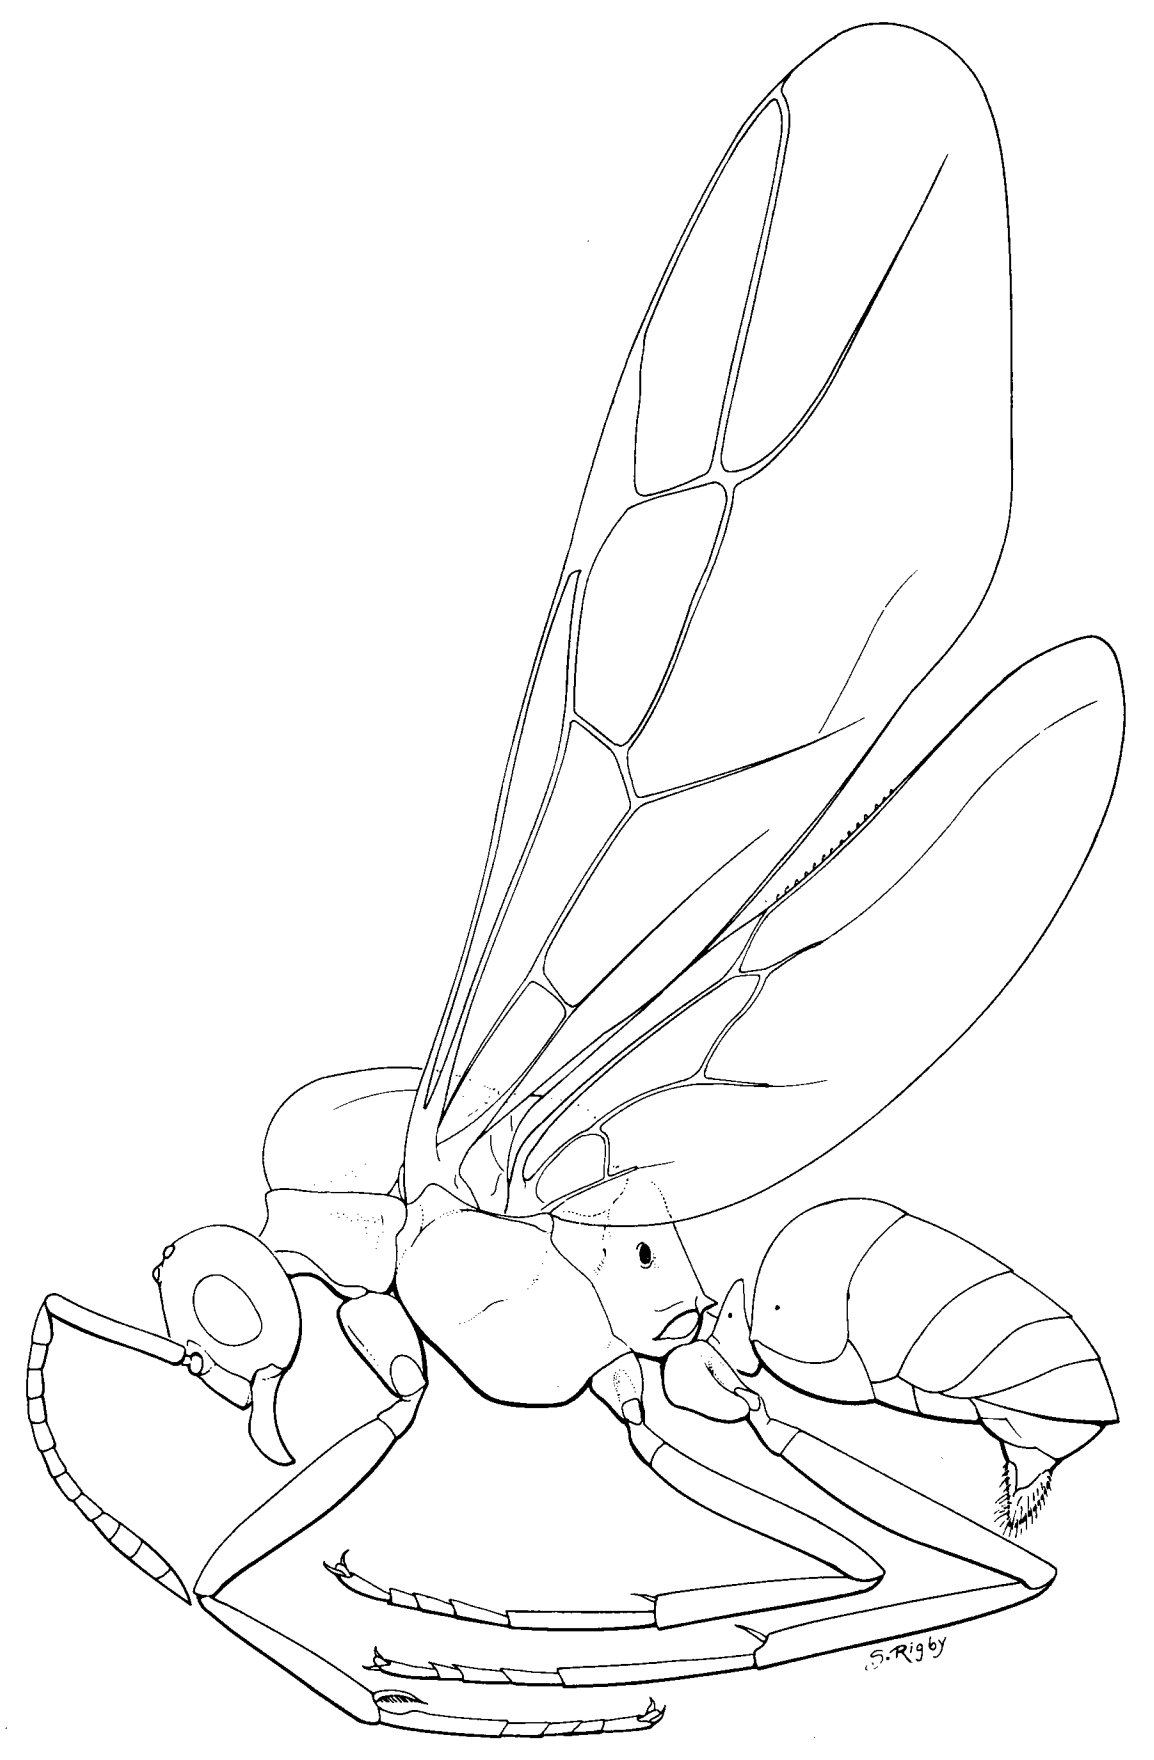
\includegraphics[width=\textwidth]{MaleFormicidHabitus}
        \caption{Male habitus \citep[][Fig. 92]{goulet1993hymenoptera}}
        \label{fig:formicid2}
    \end{subfigure}
    \caption{Formicidae}\label{fig:formicids}
\end{figure}

\subsubsection{Pompilidae (spider wasps)}
\begin{itemize}
\item antennal segments distinctly separated and often curled in dead specimens
\item pronotum with posterolateral apex rounded anterior to tegula
\item mesopleuron usually with oblique sulcus (Figure \ref{fig:pompilid2})
\item mesosoma usually laterally flattened (\textit{i.e.}, mesosoma higher than wide in anterior or posterior view)
\item hind wing without distinct claval lobe but with distinct jugal lobe (Figure \ref{fig:pompilid3})
\item legs usually conspicuously elongate, spiny 
\end{itemize}

\begin{figure}[ht!]
    \centering
    \begin{subfigure}[ht!]{0.32\textwidth}
        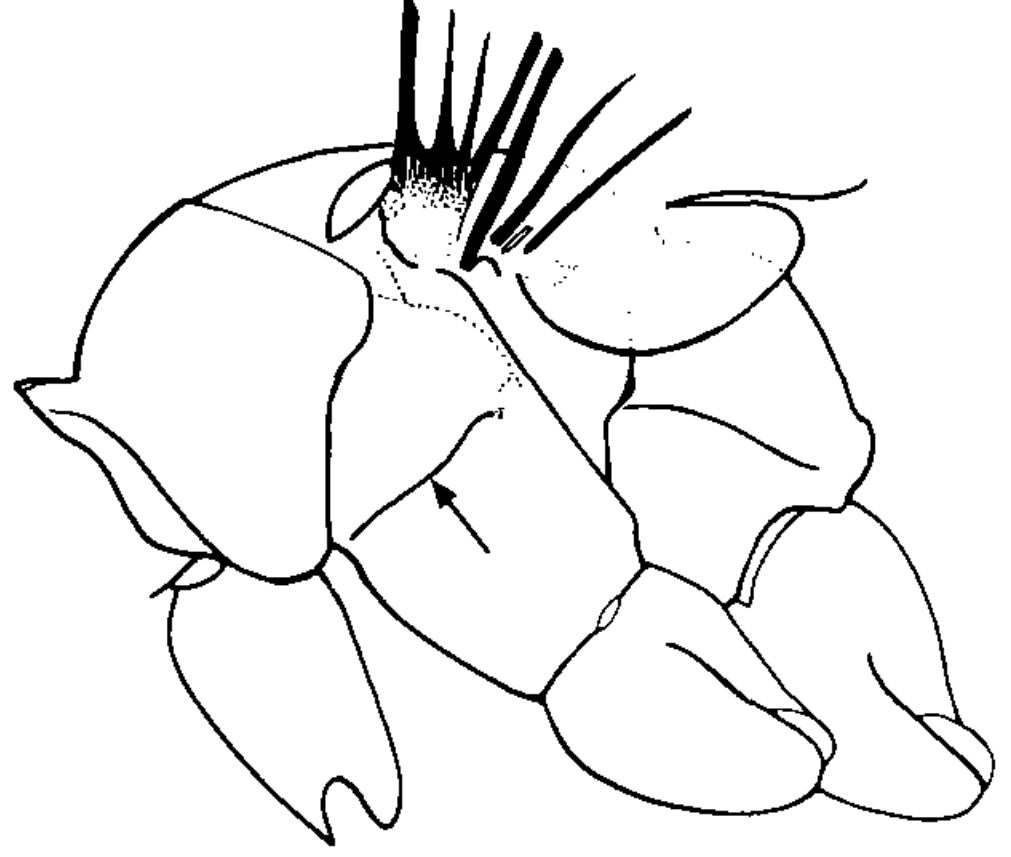
\includegraphics[width=\textwidth]{PompilidMesosoma}
        \caption{Mesosoma, with mesopleural sulcus (arrow) \citep[][pg. 170]{goulet1993hymenoptera}}
        \label{fig:pompilid2}
    \end{subfigure}
    \qquad
    \begin{subfigure}[ht!]{0.38\textwidth}
        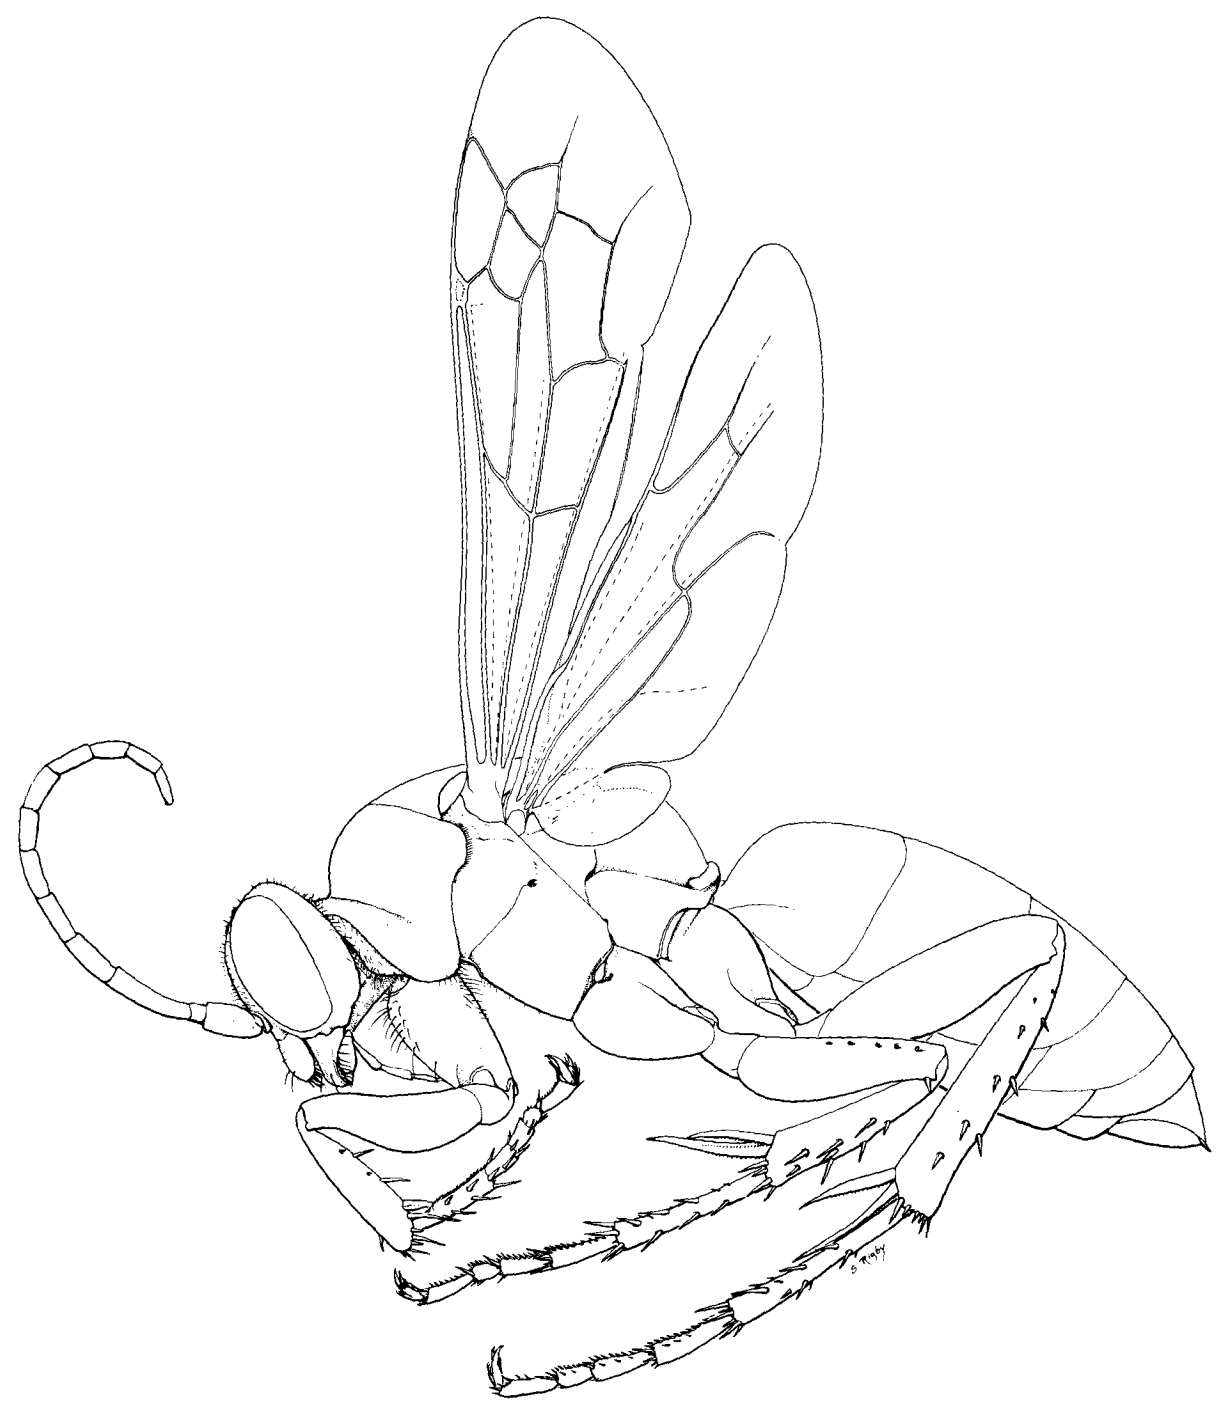
\includegraphics[width=\textwidth]{PompilidHabitus}
        \caption{Habitus \citep[][Fig. 71]{goulet1993hymenoptera}}
        \label{fig:pompilid3}
    \end{subfigure}
    \caption{Pompilidae}\label{fig:pompilid}
\end{figure}

\subsubsection{Scoliidae}
\begin{itemize}
\item eye with inner margin deeply emarginated (``notched'')
\item pronotum with posterodorsal margin U-shaped 
\item pronotum posterolateral apex truncate and weakly produced above anterior margin of tegula
\item mesocoxae and metacoxa widely separated 
\item wings with dense fine longitudinal wrinkles near apices (Figure \ref{fig:scoliid1})
\item hind wing without distinct claval lobe but with distinct jugal lobe
female usually with mesotibia and metatibia stout and spiny. 
\item metasomal sternum 1 separated from sternum 2 by a deep constriction 
\end{itemize}

\begin{figure}[ht!]
    \centering
    \begin{subfigure}[ht!]{0.28\textwidth}
        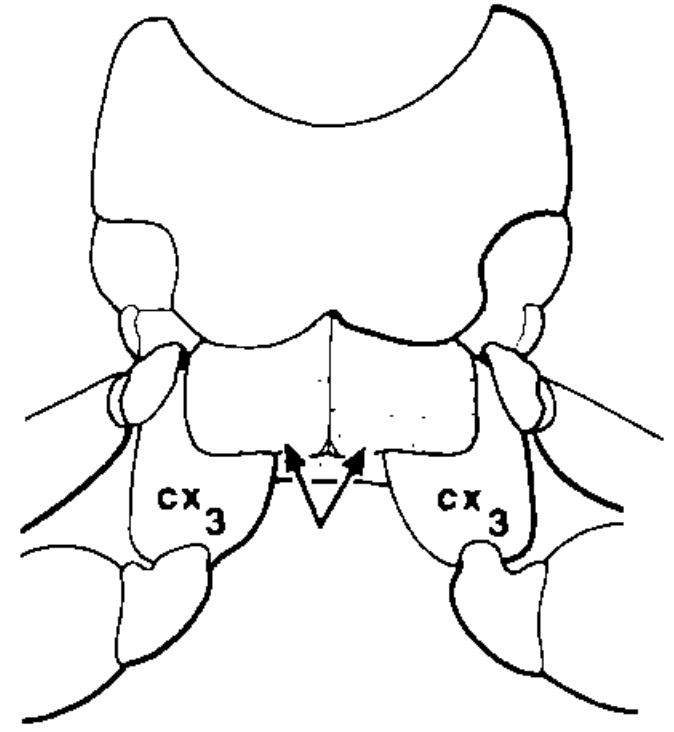
\includegraphics[width=\textwidth]{ScoliidMesosoma}
        \caption{Mesosoma in ventral view \citep[][pg. 162]{goulet1993hymenoptera}; cx3 = metacoxa}
        \label{fig:scoliid1}
    \end{subfigure}
    \qquad
    \begin{subfigure}[ht!]{0.38\textwidth}
        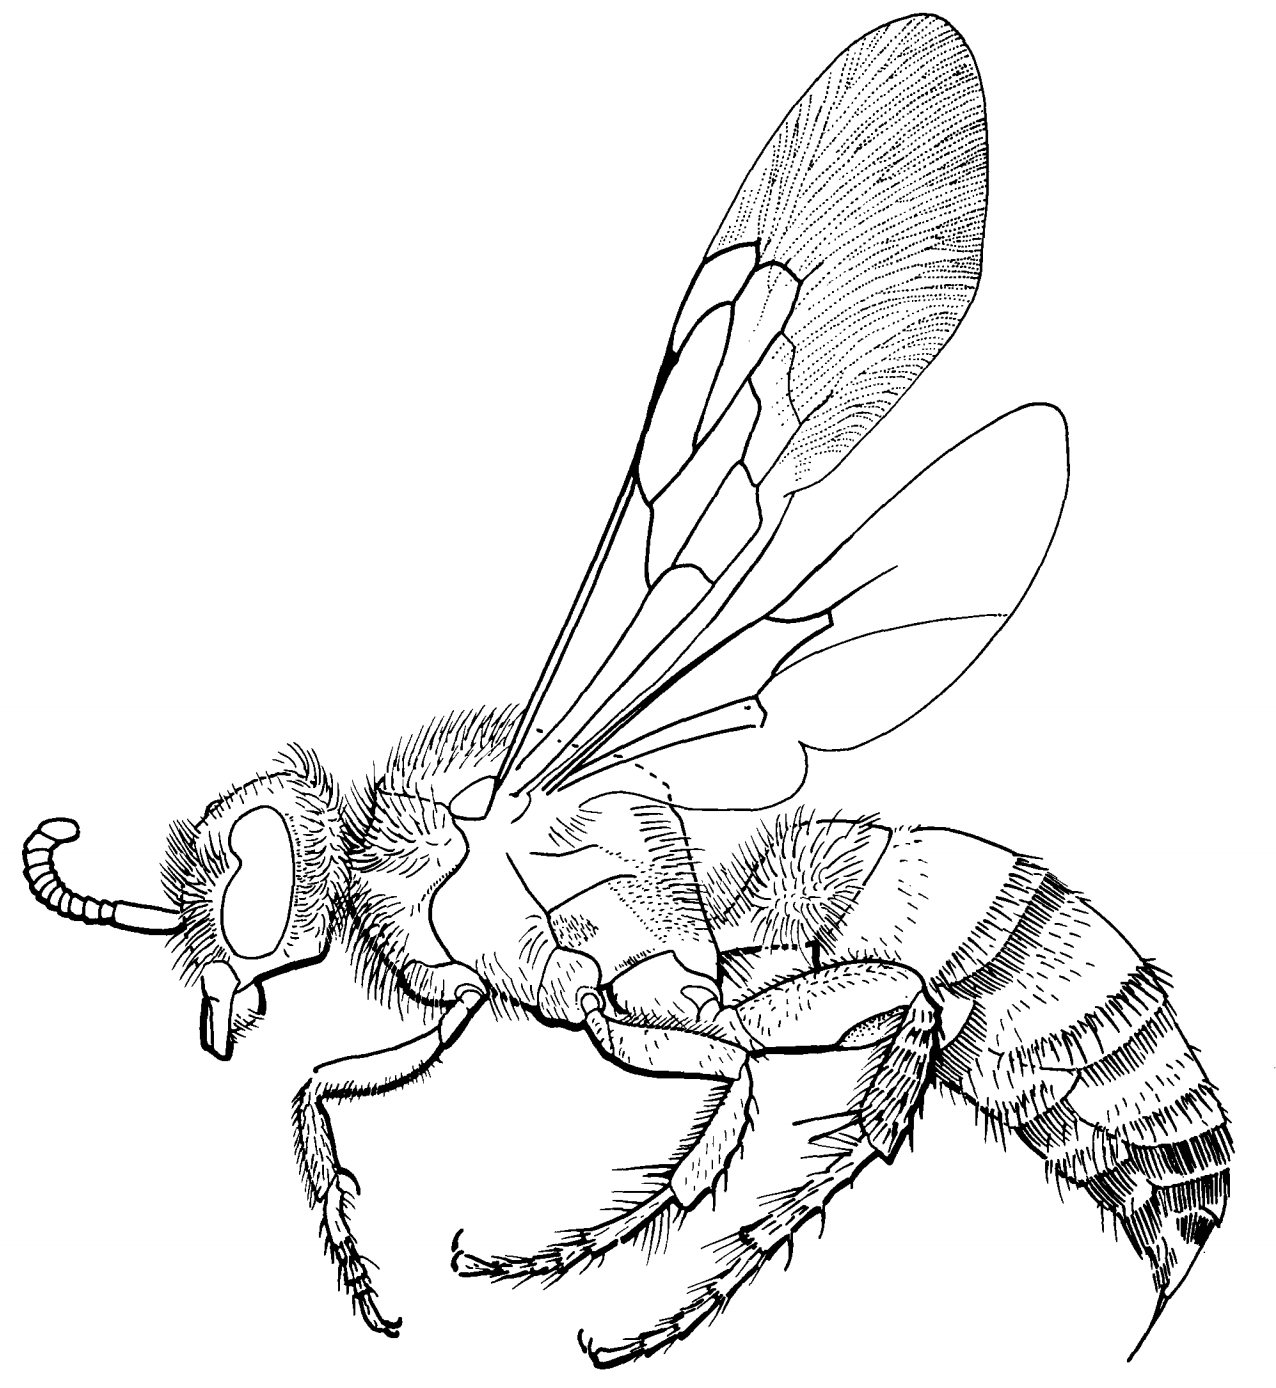
\includegraphics[width=\textwidth]{ScoliidHabitus}
        \caption{Habitus \citep[][Fig. 78]{goulet1993hymenoptera}}
        \label{fig:scoliid2}
    \end{subfigure}
    \caption{Scoliidae}\label{fig:scoliids}
\end{figure}

\subsubsection{Vespidae}
\begin{itemize}
\item eye with inner margin deeply emarginated 
\item pronotum posterodorsal margin V-shaped, and with pronotum posterolateral apex acute and strongly produced above anterior margin of tegula
\item fore wing almost always longitudinally folded when at rest 
\item hind wing without distinct claval lobe, and usually with distinct jugal lobe
\item posterior (inner) spur of metatibia weakly modified as a calcar 
\item metasomal sternum 1 separated from sternum 2 by a deep constriction
\end{itemize}

\noindent{}Many vespids are highly eusocial (You've probably encountered yellowjackets or bald-faced hornets here in Pennsylvania). Do you see any morphological evidence that these species are eusocial? Recall the question above for Formicidae.\\

\begin{figure}[ht!]
    \centering
    \begin{subfigure}[ht!]{0.25\textwidth}
        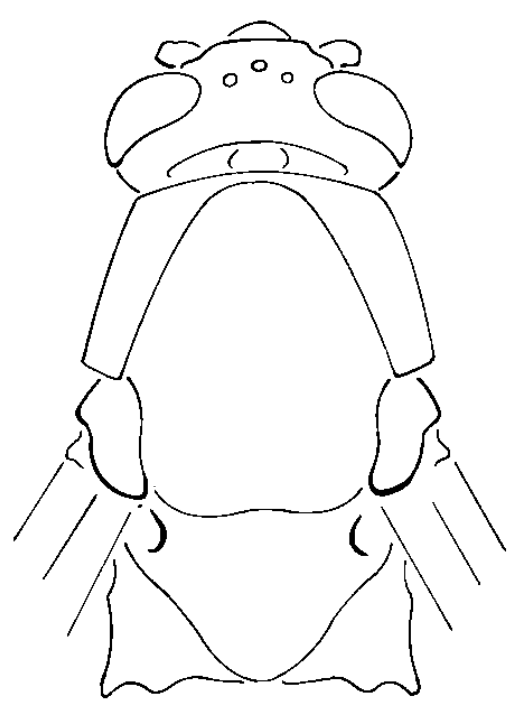
\includegraphics[width=\textwidth]{VespidMesosoma}
        \caption{Dorsal head and mesosoma \citep[][pg. 215]{goulet1993hymenoptera}}
        \label{fig:vespid1}
    \end{subfigure}
    \hfill
    \begin{subfigure}[ht!]{0.2\textwidth}
        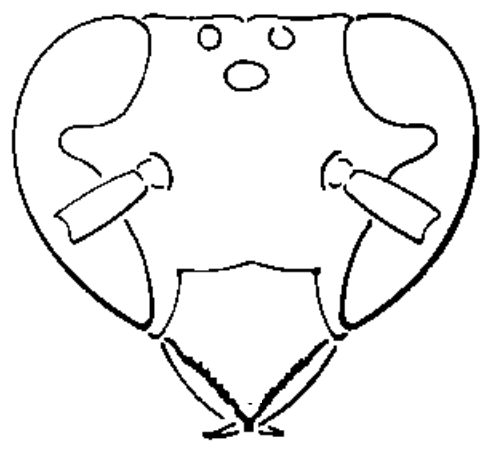
\includegraphics[width=\textwidth]{VespidHead}
        \caption{Anterior head \citep[][pg. 214]{goulet1993hymenoptera}}
        \label{fig:vespid2}
    \end{subfigure}
    \hfill
    \begin{subfigure}[ht!]{0.45\textwidth}
        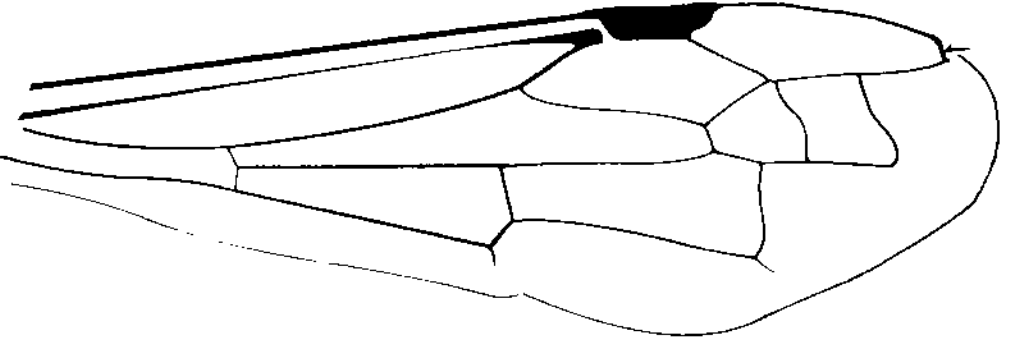
\includegraphics[width=\textwidth]{VespidWing}
        \caption{Fore wing \citep[][pg. 214]{goulet1993hymenoptera}}
        \label{fig:vespid3}
    \end{subfigure}
    \caption{Vespidae}\label{fig:vespids}
\end{figure}
\FloatBarrier

\noindent{}Now we're in Apoidea. This taxon comprises four families of spheciform wasps (we'll look at two), which are mostly predators of other insects, and seven to nine families of bees (Anthophila; we'll look at four bee families), which collect pollen. \\

\subsubsection{Sphecidae (thread-waisted, hunting wasps)}
\begin{itemize}
\item plumose, branched setae absent
\item hind leg basitarsus as wide as subsequent tarsomeres 
\item metasoma petiolate (Figure \ref{fig:sphecid1})
\item first metasomal segment tube-like (sternum and tergum fused)
\end{itemize}

\begin{figure}[ht!]
    \centering
    \begin{subfigure}[ht!]{0.45\textwidth}
        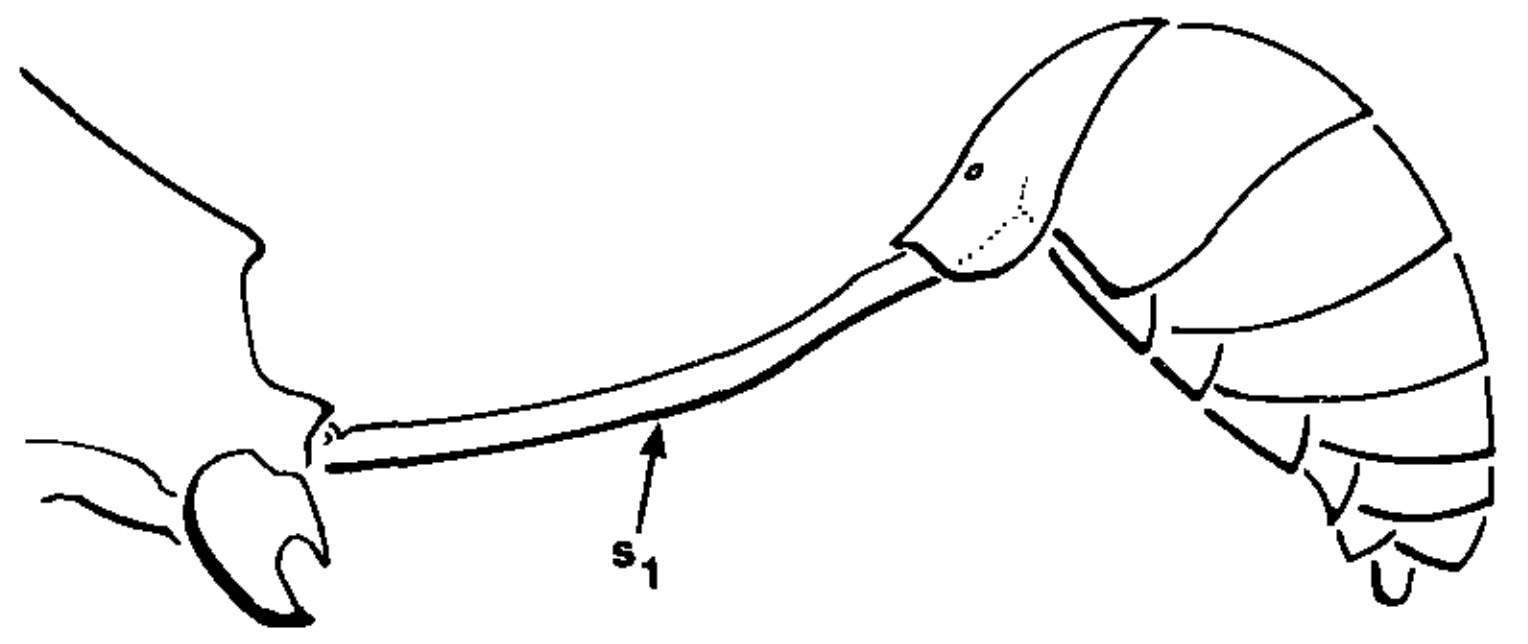
\includegraphics[width=\textwidth]{SphecidMetasoma}
        \caption{Mesasoma; s1 = sternite 1}
        \label{fig:sphecid1}
    \end{subfigure}
    \qquad
    \begin{subfigure}[ht!]{0.45\textwidth}
        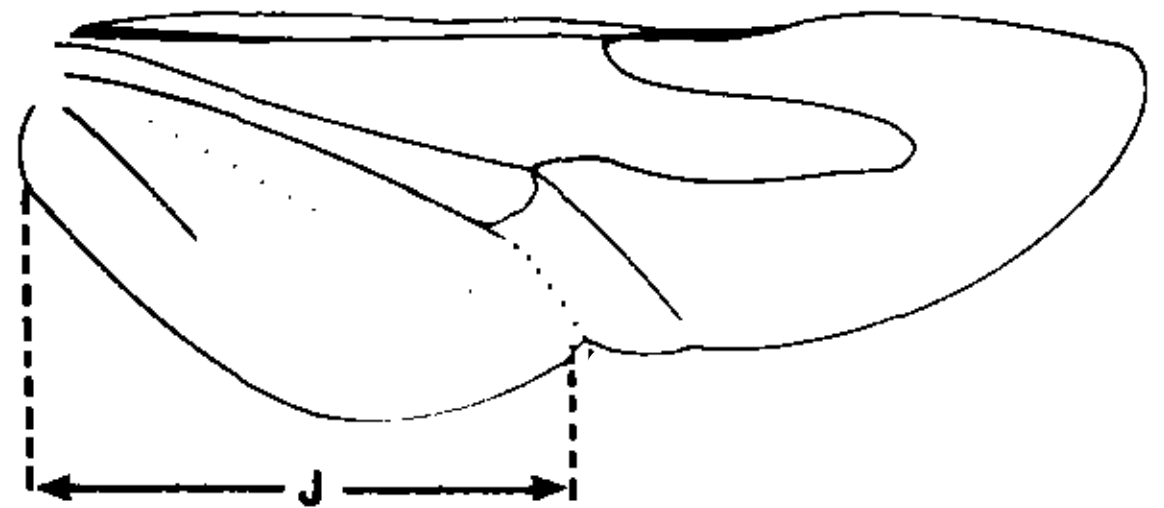
\includegraphics[width=\textwidth]{SphecidWing}
        \caption{Hind wing; J = jugal lobe}
        \label{fig:sphecid2}
    \end{subfigure}
    \caption{Sphecidae \citep[][pg. 281]{goulet1993hymenoptera}}\label{fig:sphecids}
\end{figure}

\subsubsection{Crabronidae (hunting wasps, aphid wasps, beewolves, cicada killers, \textit{etc}.)}
\begin{itemize}
\item plumose, branched setae absent
\item hind leg basitarsus as wide as subsequent tarsomeres 
\item tergum and sternum distinctly separated on metasomal segment 1; sometimes forming tube-like petiole
\item often determined through the process of elimination
\end{itemize}

\begin{figure}[ht!]
    \centering
    \begin{subfigure}[ht!]{0.4\textwidth}
        \includegraphics[width=\textwidth]{CrabronidHabitus1}
        \caption{Pemphredoninae habitus \citep[][Fig. 99]{goulet1993hymenoptera}}
        \label{fig:crabronid1}
    \end{subfigure}
    \qquad
    \begin{subfigure}[ht!]{0.4\textwidth}
        \includegraphics[width=\textwidth]{CrabronidHabitus2}
        \caption{Larrinae habitus \citep[][Fig. 102]{goulet1993hymenoptera}}
        \label{fig:crabronid2}
    \end{subfigure}
    \caption{Crabronidae}\label{fig:crabronids}
\end{figure}
\FloatBarrier

\noindent{}The remaining hymenopteran families are classified in \textbf{Anthophila} (bees). All have branched setae on the body and usually have (in females) some kind of pollen-carrying structure on the hind legs or abdomen.

\subsubsection{Halictidae (sweat bees)}
\begin{itemize}
\item hind leg basitarsus much wider than subsequent tarsomeres 
\item face with one subantennal suture
\item proboscis short
\item jugal lobe of hind wing long
\item basal vein of fore wing strongly arched (Figure \ref{fig:halict1})
\item small to medium-sized, often metallic
\end{itemize}

\begin{figure}[ht!]
    \centering
    \begin{subfigure}[ht!]{0.26\textwidth}
        \includegraphics[width=\textwidth]{HalictidFace}
        \caption{Face \citep[][pg. 315]{goulet1993hymenoptera}}
        \label{fig:halict1}
    \end{subfigure}
    \qquad
    \begin{subfigure}[ht!]{0.4\textwidth}
        \includegraphics[width=\textwidth]{HalictidHabitus}
        \caption{Habitus \citep[][Fig. 118]{goulet1993hymenoptera}}
        \label{fig:halict2}
    \end{subfigure}
    \caption{Halictidae}\label{fig:halictidae}
\end{figure}

\subsubsection{Andrenidae (mining bees)}
\begin{itemize}
\item proboscis short
\item face with two subantennal sutures (Fig. \ref{fig:andrenid1}, double arrow) and often with facial foveae (Fig. \ref{fig:andrenid1}, single arrow)
\item jugal lobe of hind wing long
\item basal vein of fore wing not strongly arched
\item small to medium-sized, often (not always!) with hairier thorax than halictids
\end{itemize}

\begin{figure}[ht!]
    \centering
    \begin{subfigure}[ht!]{0.26\textwidth}
        \includegraphics[width=\textwidth]{AndrenidFace}
        \caption{Head in anterior view \citep[][pg. 313]{goulet1993hymenoptera}}
        \label{fig:andrenid1}
    \end{subfigure}
    \qquad
    \begin{subfigure}[ht!]{0.38\textwidth}
        \includegraphics[width=\textwidth]{AndrenidHabitus}
        \caption{Habitus \citep[][Fig. 116]{goulet1993hymenoptera}}
        \label{fig:andrenid2}
    \end{subfigure}
    \caption{Andrenidae}\label{fig:andrenids}
\end{figure}

\subsubsection{Megachilidae (mason, leafcutter bees, \textit{etc}.)}
\begin{itemize}
\item proboscis rather long
\item jugal lobe of hind wing short
\item fore wing with two submarginal cells, usually equal in length
\item females with scopa (pollen carrier) on ventral surface of metasoma
\item variable in color and shape, but often stouter or ``chunkier'' than other bees
\end{itemize}

\begin{figure}[ht!]
    \centering
     \begin{subfigure}[ht!]{0.42\textwidth}
        \includegraphics[width=\textwidth]{MegachilidHabitus}
        \caption{Habitus \citep[][Fig. 116]{goulet1993hymenoptera}}
        \label{fig:megachilid1}
    \end{subfigure}
   \qquad
    \begin{subfigure}[ht!]{0.32\textwidth}
        \includegraphics[width=\textwidth]{ApidHabitus}
        \caption{Habitus \citep[][Fig. 123]{goulet1993hymenoptera}}
        \label{fig:apid1}
    \end{subfigure}
    \caption{}\label{fig:notused}
\end{figure}

\subsubsection{Apidae (cuckoo, nomad, carpenter, bumble, honey bees, \textit{etc}.)}
\begin{itemize}
\item tongue long, maxillary palps vestigial
\item jugal lobe of hind wing usually absent
\item fore wing with three submarginal cells
\item hind tibiae usually with a scopa used to carry pollen
\end{itemize}

\noindent{}As you have now seen, almost all bees are covered in plumose or branched setae and have special structures for carrying pollen. (Note: There are some species of cleptoparasitic bees that lack these structures.) Take a close look at the setae. Are they uniform in size and shape? How many specialized structures can you find on the body that you hypothesize might be involved in pollen collection? Based on the morphology, can you envision how pollen collection works from a behavioral perspective?

\FloatBarrier
% adding bibliography here
\bibliographystyle{apalike}
\bibliography{bib}

\end{document}

\subsubsection{Cimbicidae (cimbicid sawflies)}
\begin{itemize}
\item antennae with less than 7 flagellomeres, club=like
\item fore wing with 2 marginal cells 
\item two veins along the anteroproximal margin of fore wing connecting pterostigma with wing base
\item first abdominal tergum extending to metacoxa and fused with metapleuron
\end{itemize}


\subsubsection{Xiphydriidae (woodwasps)}
\begin{itemize}
\item antennae with \textgreater{}10 flagellomeres
\item mesonotum is divided by a straight transverse groove (Figure \ref{fig:xyiphid1})
\item two veins along the anteroproximal margin of fore wing connecting pterostigma with wing base
\end{itemize}


\subsubsection{Stephanidae}%replace with orussidae?
\begin{itemize}
\item head globular, with crown of ``teeth'' around median ocellus
\end{itemize}
\noindent{}These insects are parasitoids of wood-boring insects. What do you think they use the crown of teeth on the head for?

\subsubsection{Proctotrupidae}
\begin{itemize}
\item antenna not elbowed, with 12 antennomeres
\item fore wing with 2 cells enclosed by tubular veins (Figure \ref{fig:proctotrupid1}); can you see them?
\item medium size, usually black or brown
\end{itemize}


\subsubsection{Platygastridae}
\begin{itemize}
\item like Scelionidae except fore wing with no veins or with only one short proximal vein distant from anterior margin
\end{itemize}
